\chapter{\ifproject%
\ifenglish Experimentation and Results\else การทดลองและผลลัพธ์\fi
\else%
\ifenglish System Evaluation\else การประเมินระบบ\fi
\fi}
\section{สถานีวัดสภาพอากาศขนาดย่อม}
   \hspace{\parindent} สถานีวัดสภาพอากาศขนาดย่อม อุปกรณ์ฮาร์ดแวร์จะต้องถูกนำมาประกอบและติดตั้งรวมกันไว้ภายในกล่องกันน้ำ เพื่อจัดระเบียบสายไฟและป้องกันความเสียหายจากสภาพแวดล้อมภายนอก เช่น ความชื้น ฝน และความร้อน ซึ่งทำให้ระบบพร้อมสำหรับการนำไปติดตั้งในพื้นที่หน้างานจริง 
   โดยภายในสถานีประกอบด้วยชุดเซ็นเซอร์หลักที่ทำหน้าที่ตรวจวัดและรวบรวมตัวแปรทางสภาพอากาศที่สำคัญ ได้แก่ เซ็นเซอร์ BME280 สำหรับวัดอุณหภูมิ ความชื้น และความกดอากาศ, เซ็นเซอร์ VEML7700 สำหรับวัดปริมาณความเข้มแสงแดด, เซ็นเซอร์ Wind Speed สำหรับวัดวัดความเร็ว, เซ็นเซอร์ Wind Direction สำหรับวัดทิศทางลม และเซ็นเซอร์ PT100 สำหรับวัดอุณหภูมิใต้แผงโซลาร์เซลล์ 
   \begin{figure}[H]
        \centering
        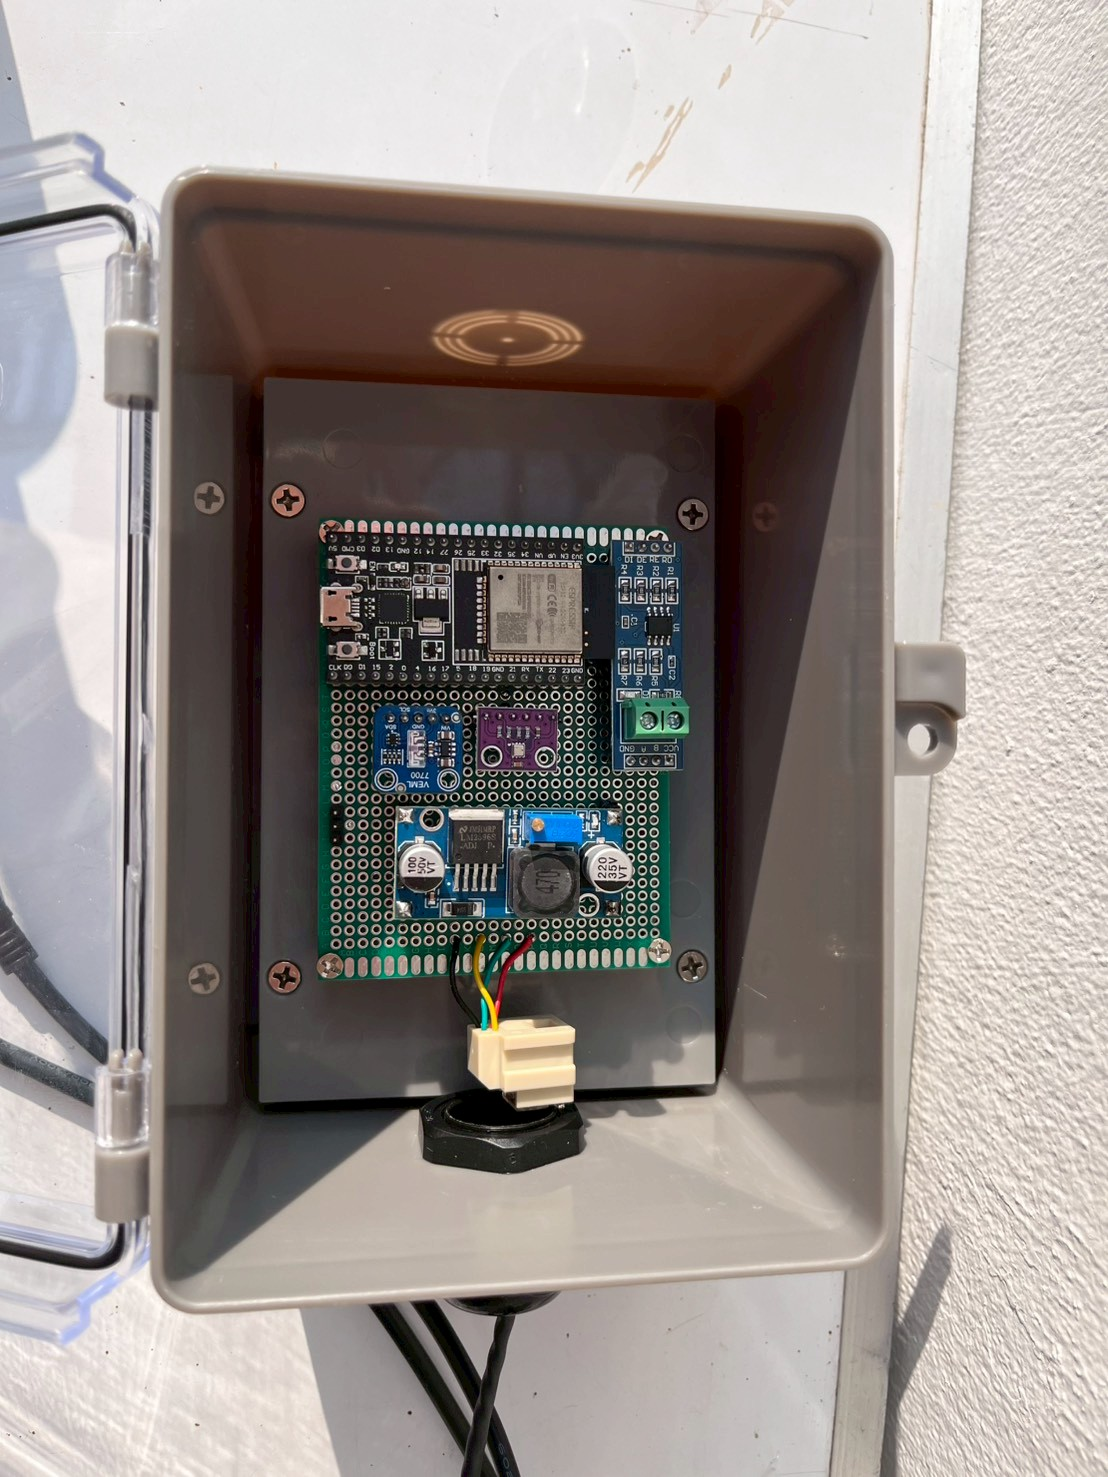
\includegraphics[width=0.7\textwidth, angle=90]{images/chapter_3/LINE_ALBUM_Station_260322_1.jpg}
        \caption{เซ็นเซอร์ BME280 และ VEML7700}
        \label{fig:BME280_VEML7700}
    \end{figure} 
    \begin{figure}[H]
        \centering
        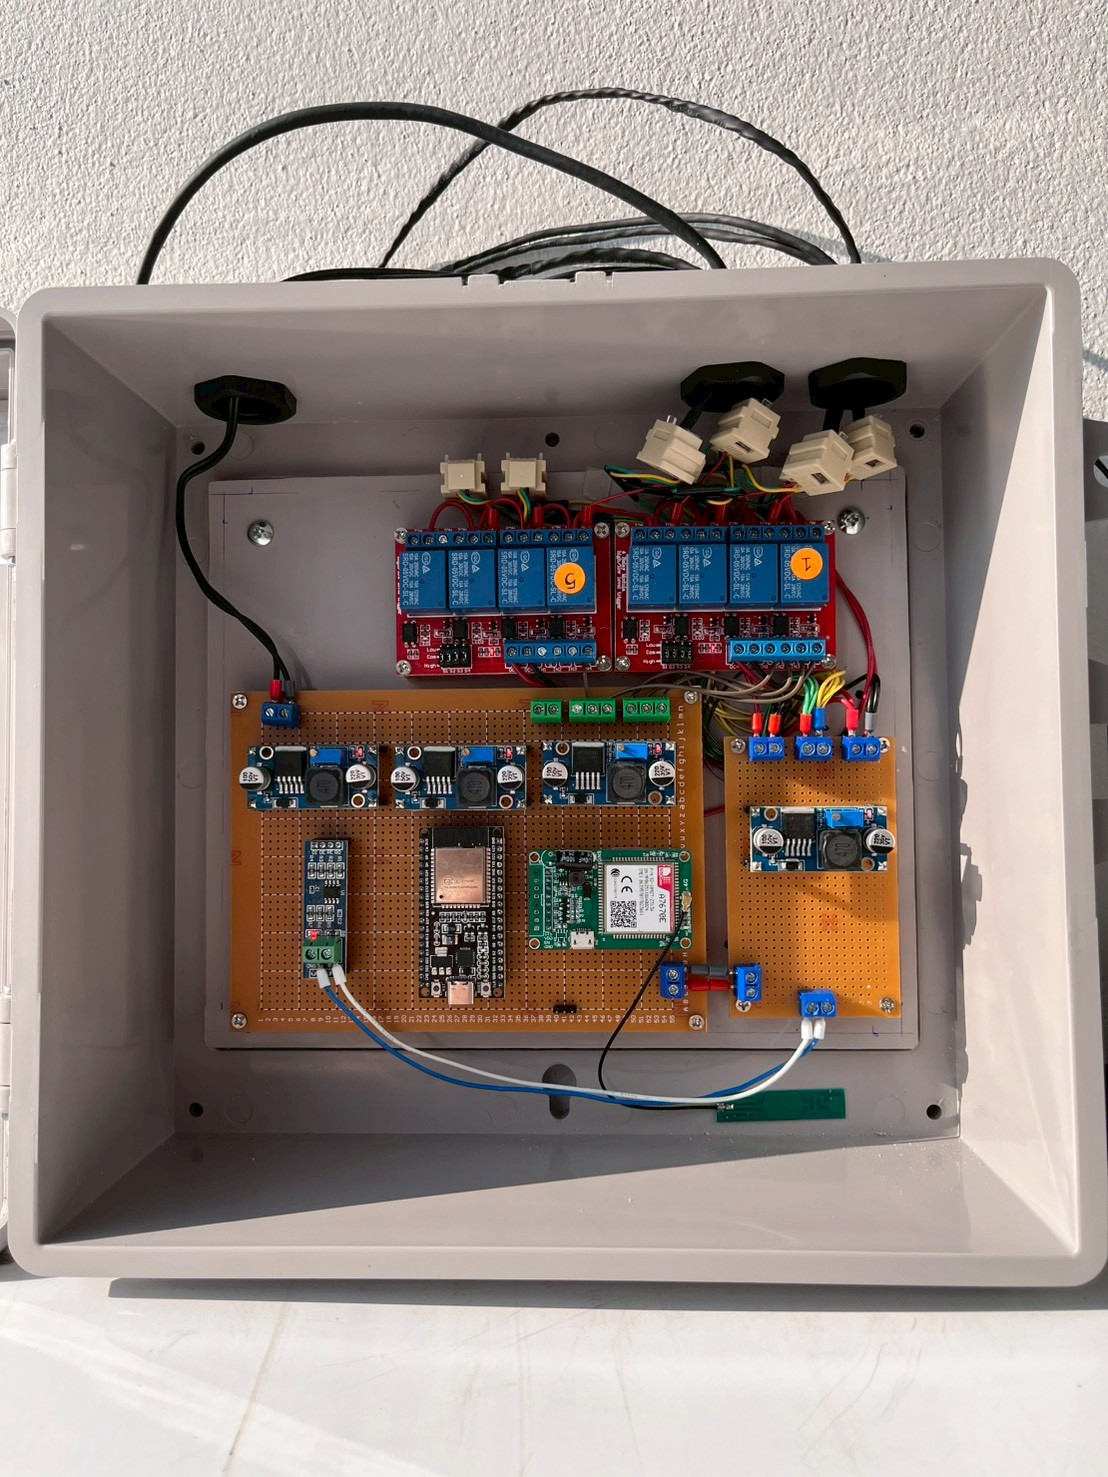
\includegraphics[width=0.7\textwidth]{images/chapter_3/main_result.jpg}
        \caption{เซ็นเซอร์ Wind Speed Wind, Direction และ PT100}
        \label{fig:Wind Speed Wind, Direction และ PT100}
    \end{figure}
     \begin{figure}[H]
        \centering
        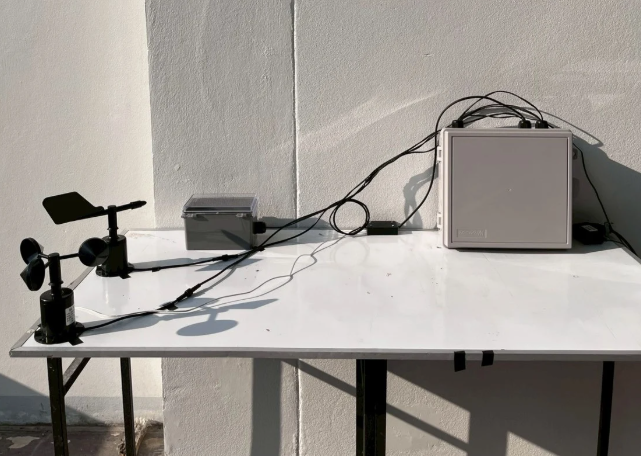
\includegraphics[width=0.7\textwidth]{picture/Hardware overview.png}
        \caption{ภาพรวมของสถานีวัดสภาพอากาศขนาดย่อม}
        \label{fig:Hardware overview}
    \end{figure}

\section{Web Dashboard}
\begin{itemize}
    \item[]\textbf{4.2.1 หน้าจอหลัก (Home)} ประกอบไปด้วยเมนู 2 เมนูคือ
    \begin{itemize}
        \item Station: เลือกสถานีวัดสภาพอากาศขนาดย่อมที่ต้องการดูข้อมูล
        \item Setting Station: เมนูสำหรับเจ้าหน้าที่ที่สามารถเข้าไปเช็คสถานะการทำงานของสถานีวัดสภาพอากาศขนาดย่อม
    \end{itemize}
    \begin{figure}[H]
        \centering
        \includegraphics[width=0.7\textwidth]{images/home.jpg}
        \caption{หน้าจอแสดงผลหลัก}
        \label{fig:Home}
    \end{figure}
    \begin{figure}[H]
        \centering
        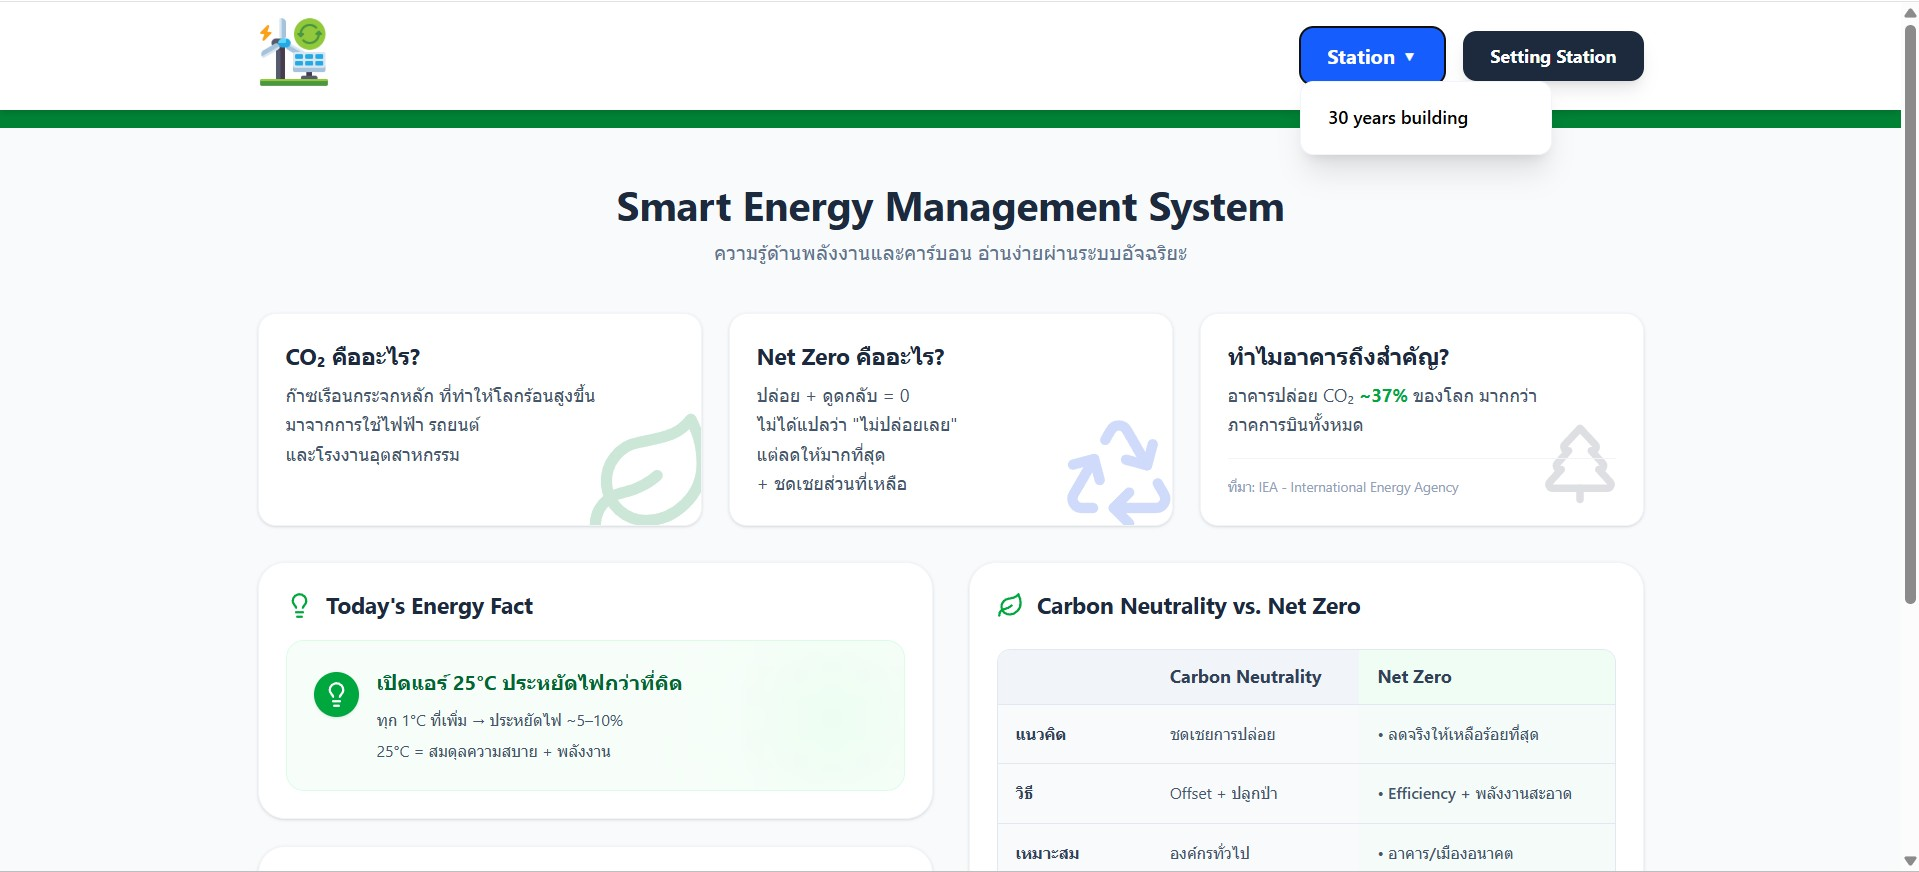
\includegraphics[width=0.7\textwidth]{images/select_station.jpg}
        \caption{หน้าจอการแสดงผลเมื่อผู้ใช้คลิกปุ่ม Station}
        \label{fig:select menu}
    \end{figure}

    \item[]\textbf{4.2.2 หน้าเมนู} หน้านี้จะแสดงข้อมูลทั้งหมดของระบบหลังจากที่ผู้ใช้เลือกปุ่ม Station ซึ่งประกอบไปด้วย
    \begin{itemize}
        \item เมนู Electric Current: แสดงกราฟการพยากรณ์ปริมาณการผลิตไฟฟ้าจากแผงโซลาร์เซลล์ซึ่งผู้ใช้สามารถเลือกวันที่ที่ต้องการดูข้อมูลได้
        \item เมนู Sunlight VS Solar Temp , Temp $&$ Humidity, Pressure, Wind Speed, Wind Direction เป็นเมนูแสดงข้อมูลที่ถูกส่งมาจากสถานีวัดสภาพอากาศขนาดย่อมรายชั่วโมง
    \end{itemize}
    \begin{figure}[H]
        \centering
        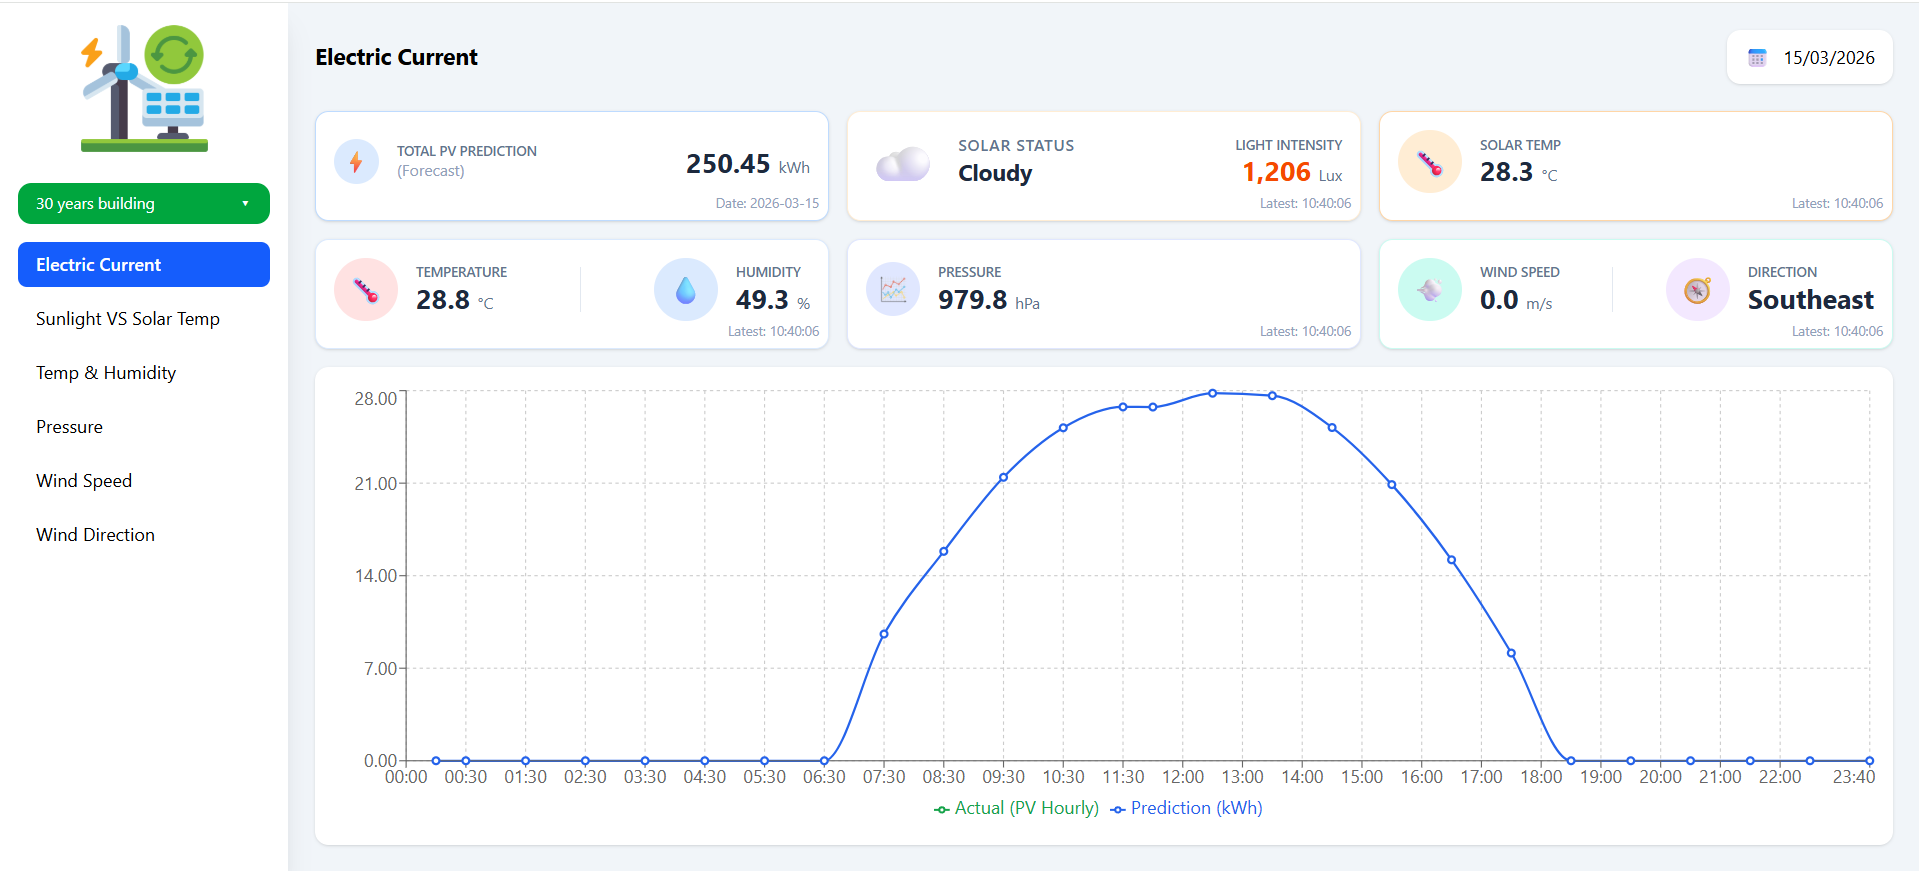
\includegraphics[width=0.7\textwidth]{images/predicgraph.png}
        \caption{หน้าจอแสดงข้อมูลสภาพอากาศและกราฟการพยากรณ์ปริมาณการผลิตไฟฟ้าจากโซลาร์เซลล์ล่วงหน้า 24 ชั่วโมง}
        \label{fig:Pradicgraph}
    \end{figure}
    \begin{figure}[H]
        \centering
        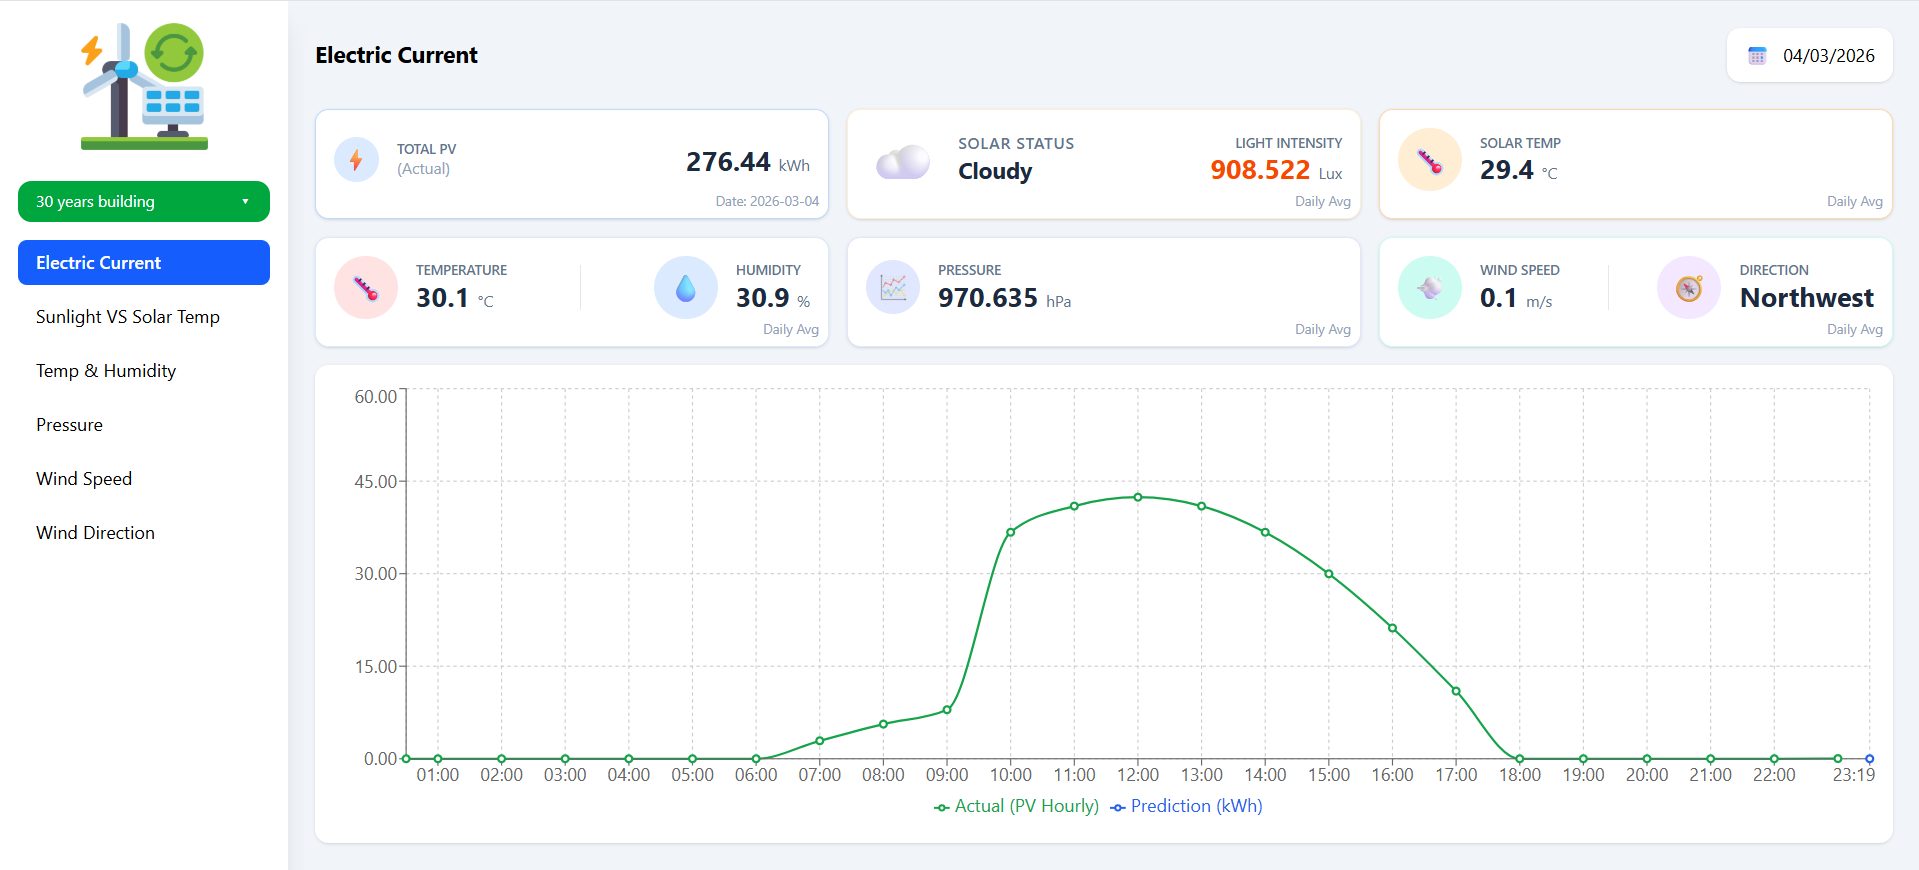
\includegraphics[width=0.7\textwidth]{images/actualgraph.png}
        \caption{หน้าจอแสดงผลเมื่อผู้ใช้เลือกเมนู Electric Current}
        \label{fig:Electric Current}
    \end{figure}
    \begin{figure}[H]
        \centering
        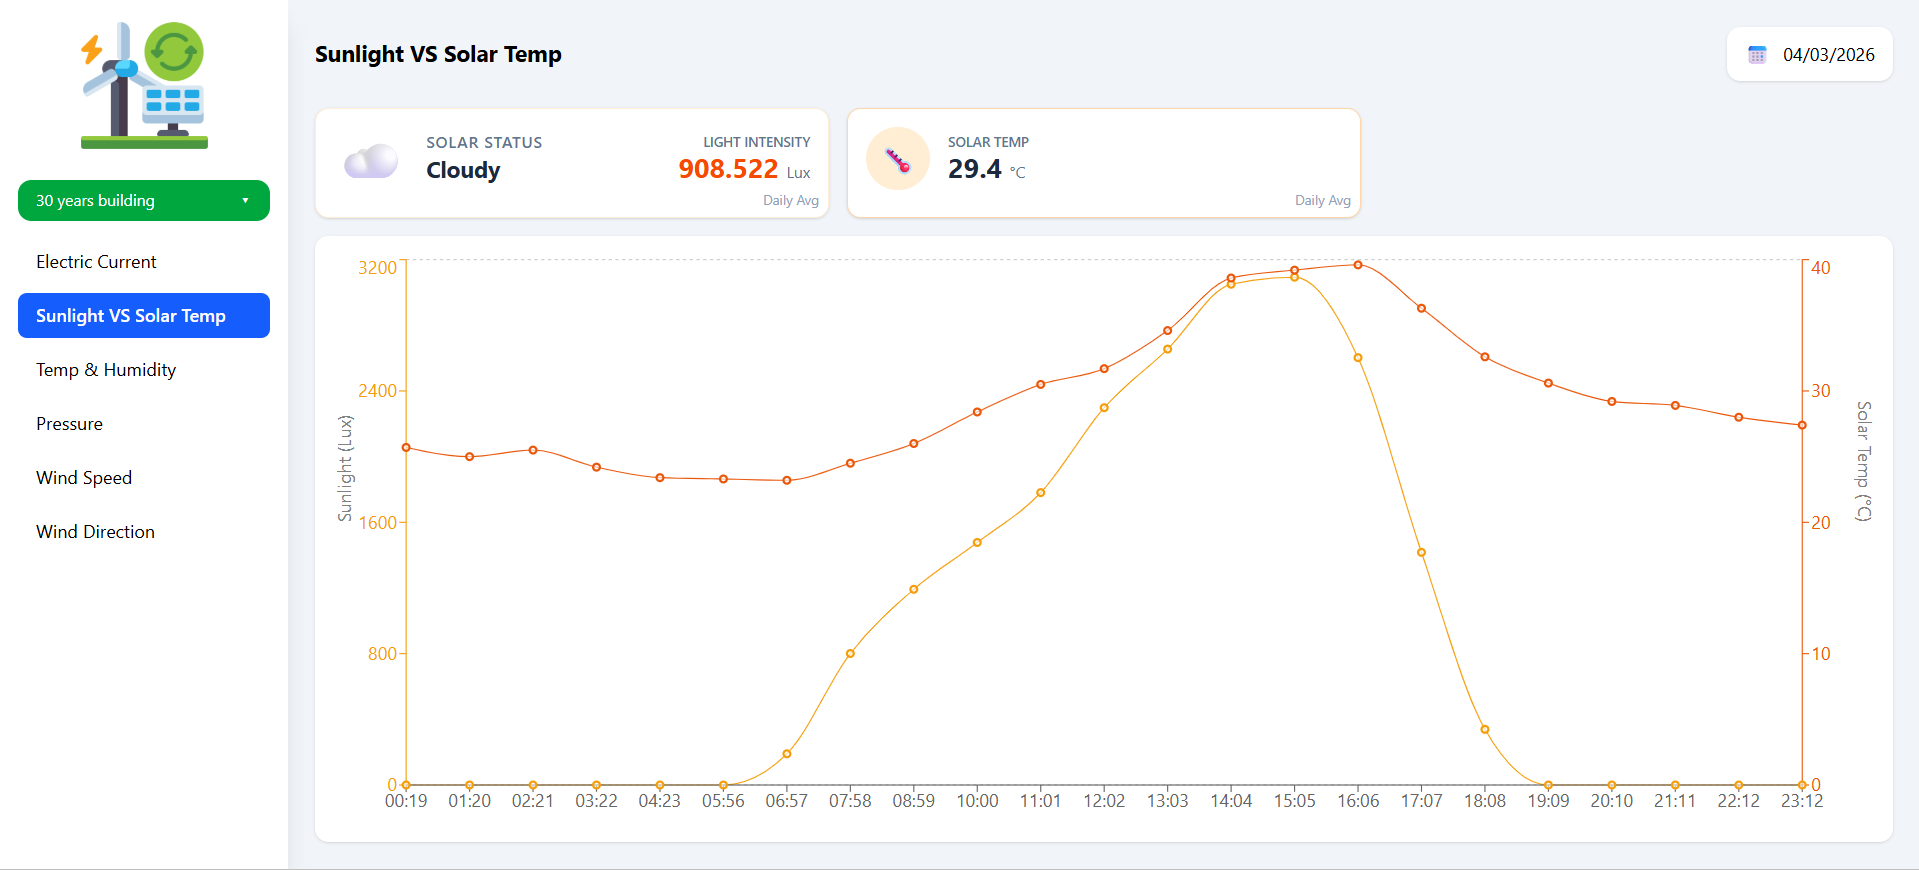
\includegraphics[width=0.7\textwidth]{images/sunlightandsolar.png}
        \caption{หน้าจอแสดงผลเมื่อผู้ใช้เลือกเมนู Sunlight VS Solar Temp}
        \label{fig:Sunlight VS Solar Temp}
    \end{figure}
    \begin{figure}[H]
        \centering
        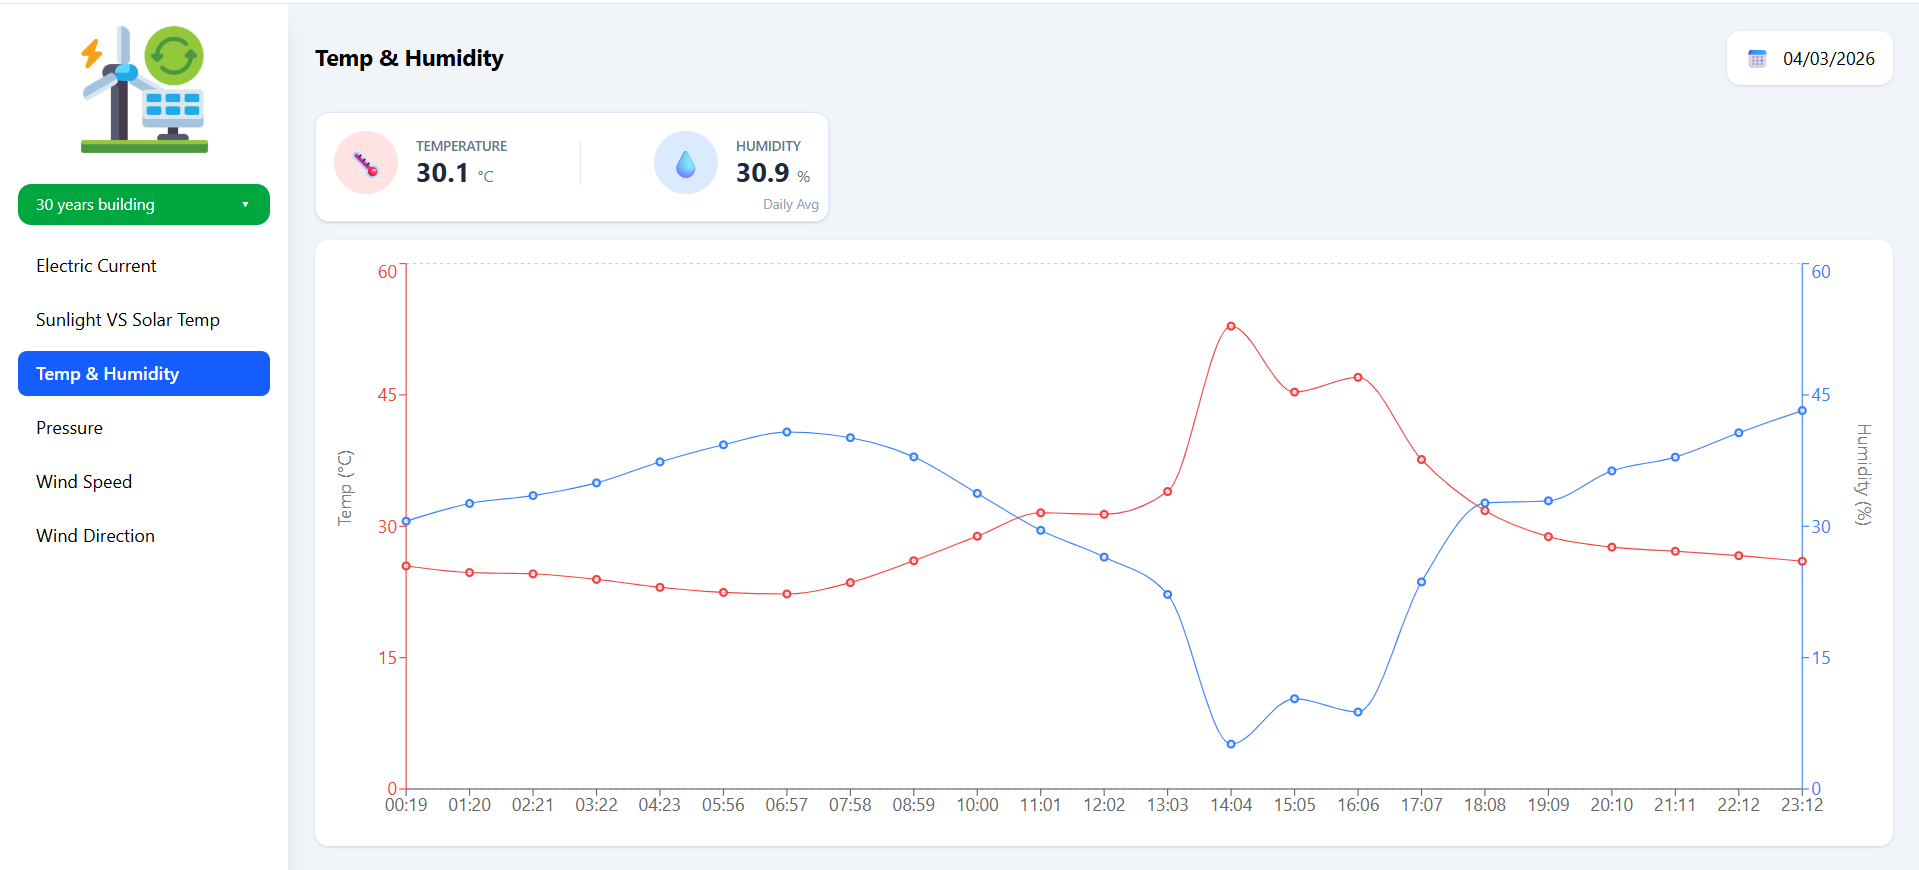
\includegraphics[width=0.7\textwidth]{images/tempandhum.png}
        \caption{หน้าจอแสดงผลเมื่อผู้ใช้เลือกเมนู Temp $&$ Humidity}
        \label{fig:Temp and Humidity}
    \end{figure}
    \begin{figure}[H]
        \centering
        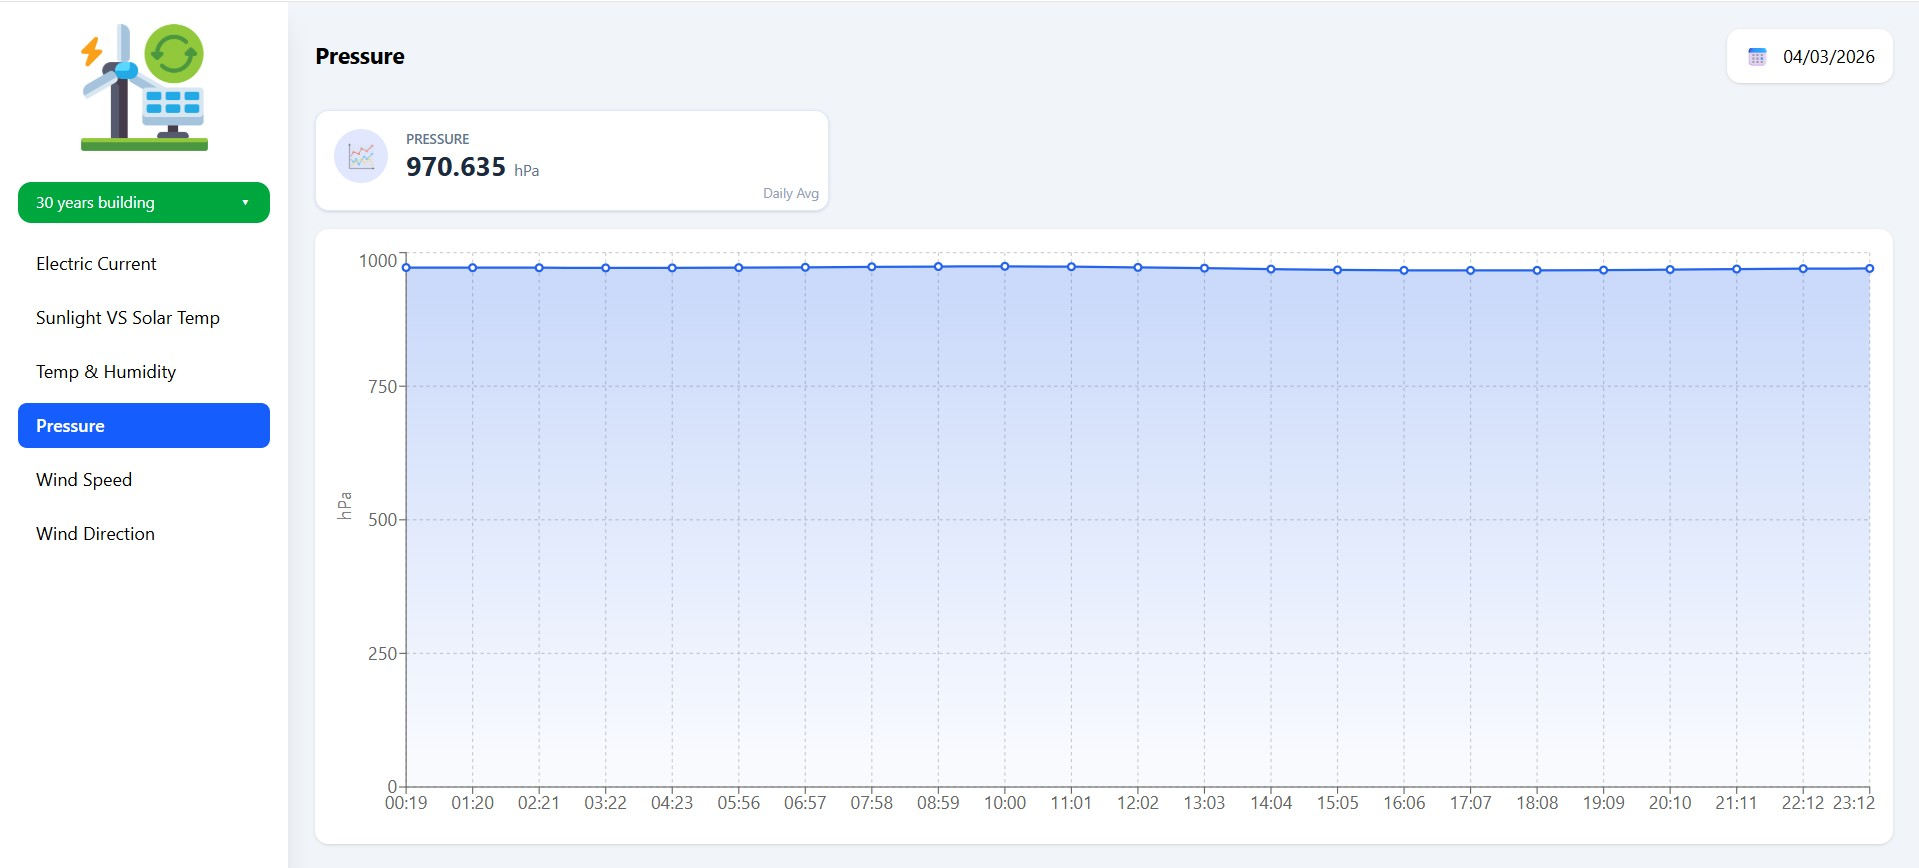
\includegraphics[width=0.7\textwidth]{images/pressure.jpg}
        \caption{หน้าจอแสดงผลเมื่อผู้ใช้เลือกเมนู Pressure}
        \label{fig:Pressure}
    \end{figure}
    \begin{figure}[H]
        \centering
        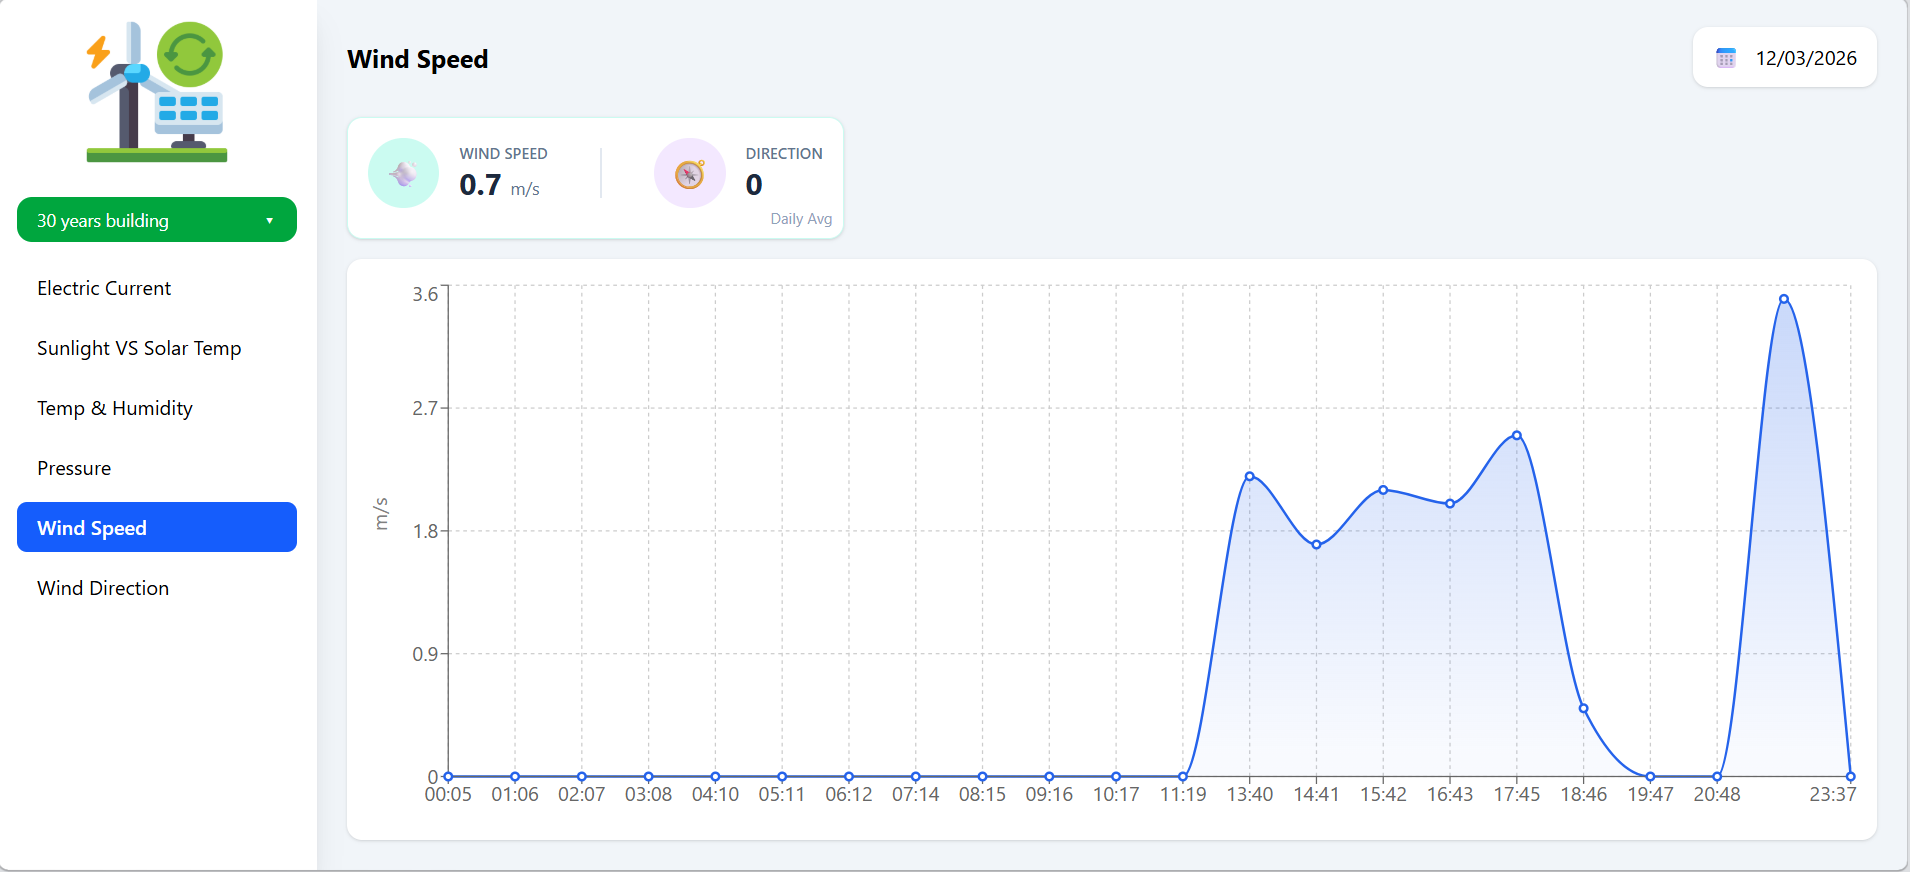
\includegraphics[width=0.7\textwidth]{picture/Wind Speed.png}
        \caption{หน้าจอแสดงผลเมื่อผู้ใช้เลือกเมนู Wind Speed}
        \label{fig:Wind Speed}
    \end{figure}
    \begin{figure}[H]
        \centering
        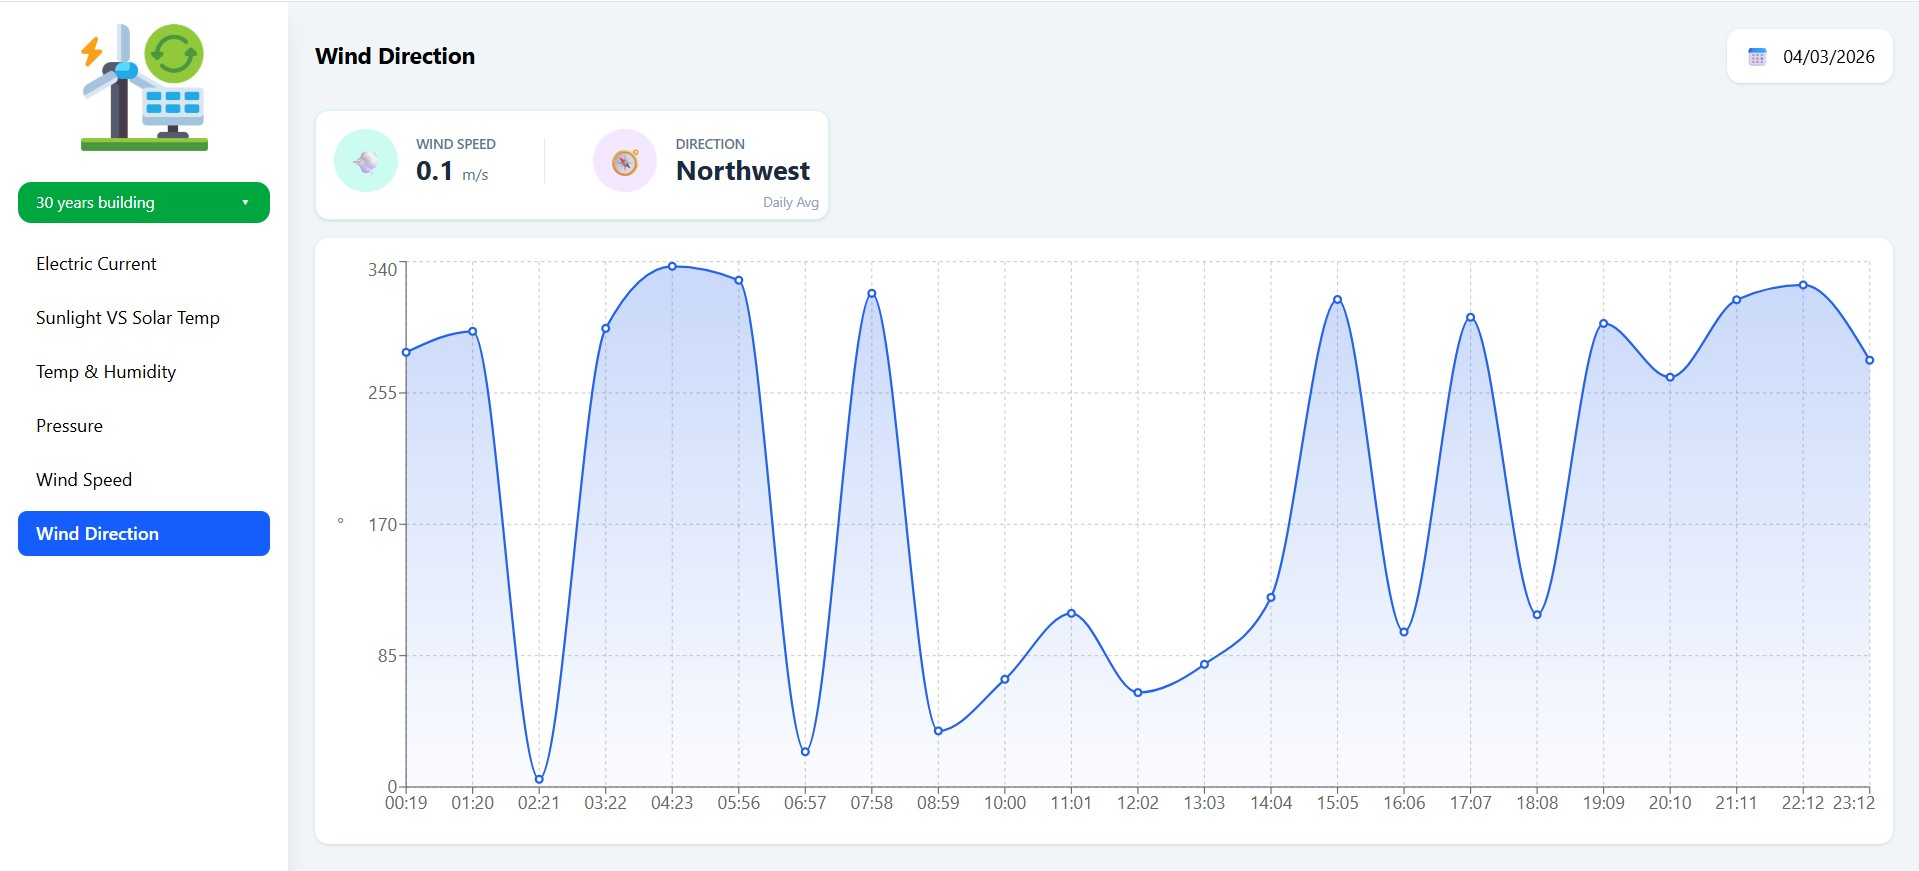
\includegraphics[width=0.7\textwidth]{images/winddirection.jpg}
        \caption{หน้าจอแสดงผลเมื่อผู้ใช้เลือกเมนู Wind Direction}
        \label{fig:Wind Direction}
    \end{figure}

    \item[]\textbf{4.2.3 หน้าสำหรับเข้าสู่ระบบ (Login)} หน้านี้มีขึ้นมาเพื่อให้เจ้าหน้าที่เท่านั้นที่สามารถเข้าถึงการทำงานของสถานีวัดสภาพอากาศขนาดย่อมเท่านั้น
    \begin{figure}[H]
        \centering
        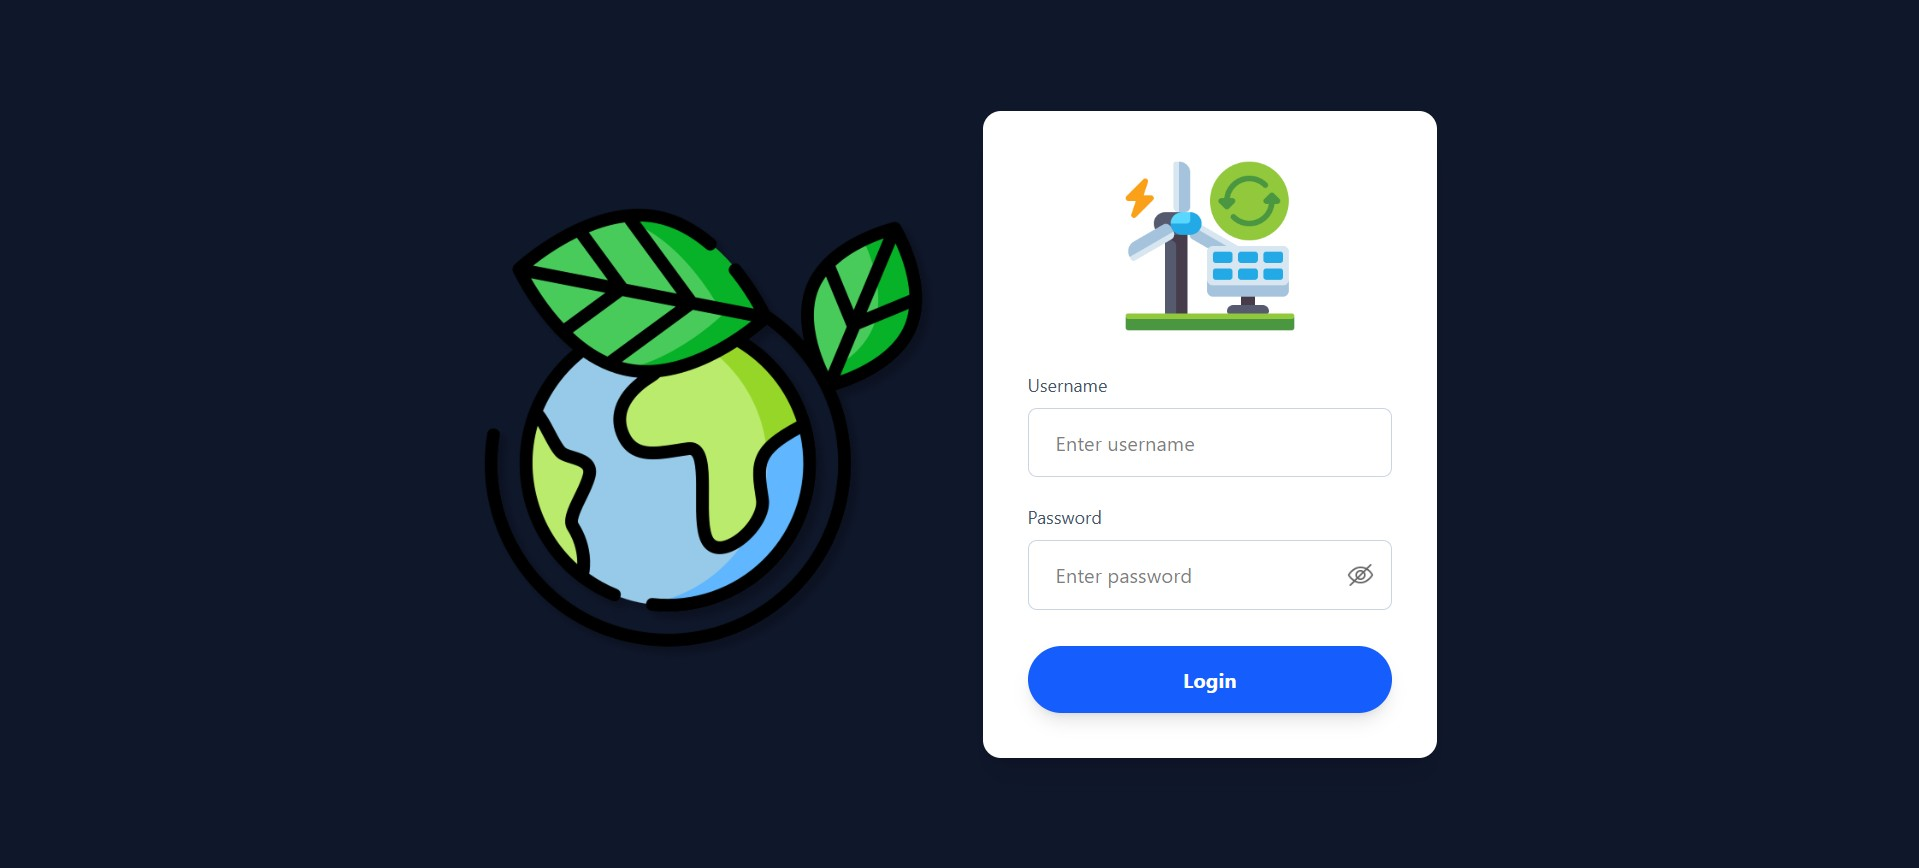
\includegraphics[width=0.7\textwidth]{images/login.jpg}
        \caption{หน้าแสดงผลเมื่อผู้ใช้เลือกเมนู Setting Station}
        \label{fig:Login}
    \end{figure}

    \item[]\textbf{4.2.4 หน้าแสดงสถานะ Status Sensor} หน้านี้มีขึ้นเพื่อติดตามสถานะการทำงานของตัววัดสถานีสภาพอากาศขนาดย่อมโดยสถานีจะต้องส่งสถานะมาทุกๆ 15 นาทีและเจ้าหน้าที่จะต้องสามารถติดตามสถานะของเซนเซอร์แต่ละตัวได้
    \begin{figure}[H]
        \centering
        
\includegraphics[width=0.7\textwidth]{statusstationOK.png} 
        \caption{สถานะการทำงานของสถานีวัดสภาพอากาศขนาดย่อมทำงานปกติ}
        \label{fig:statusstationOK}
        \end{figure}
    \begin{figure}[H]
        \centering
        
\includegraphics[width=0.7\textwidth]{statusstationNG.png} 
        \caption{สถานะการทำงานของสถานีวัดสภาพอากาศขนาดย่อมทำงานผิดปกติ}
        \label{fig:statusstationNG}
        \end{figure}
\end{itemize}

\subsection{การวิเคราะห์กราฟ Actual vs Predicted}

\begin{figure}[H]
    \centering
    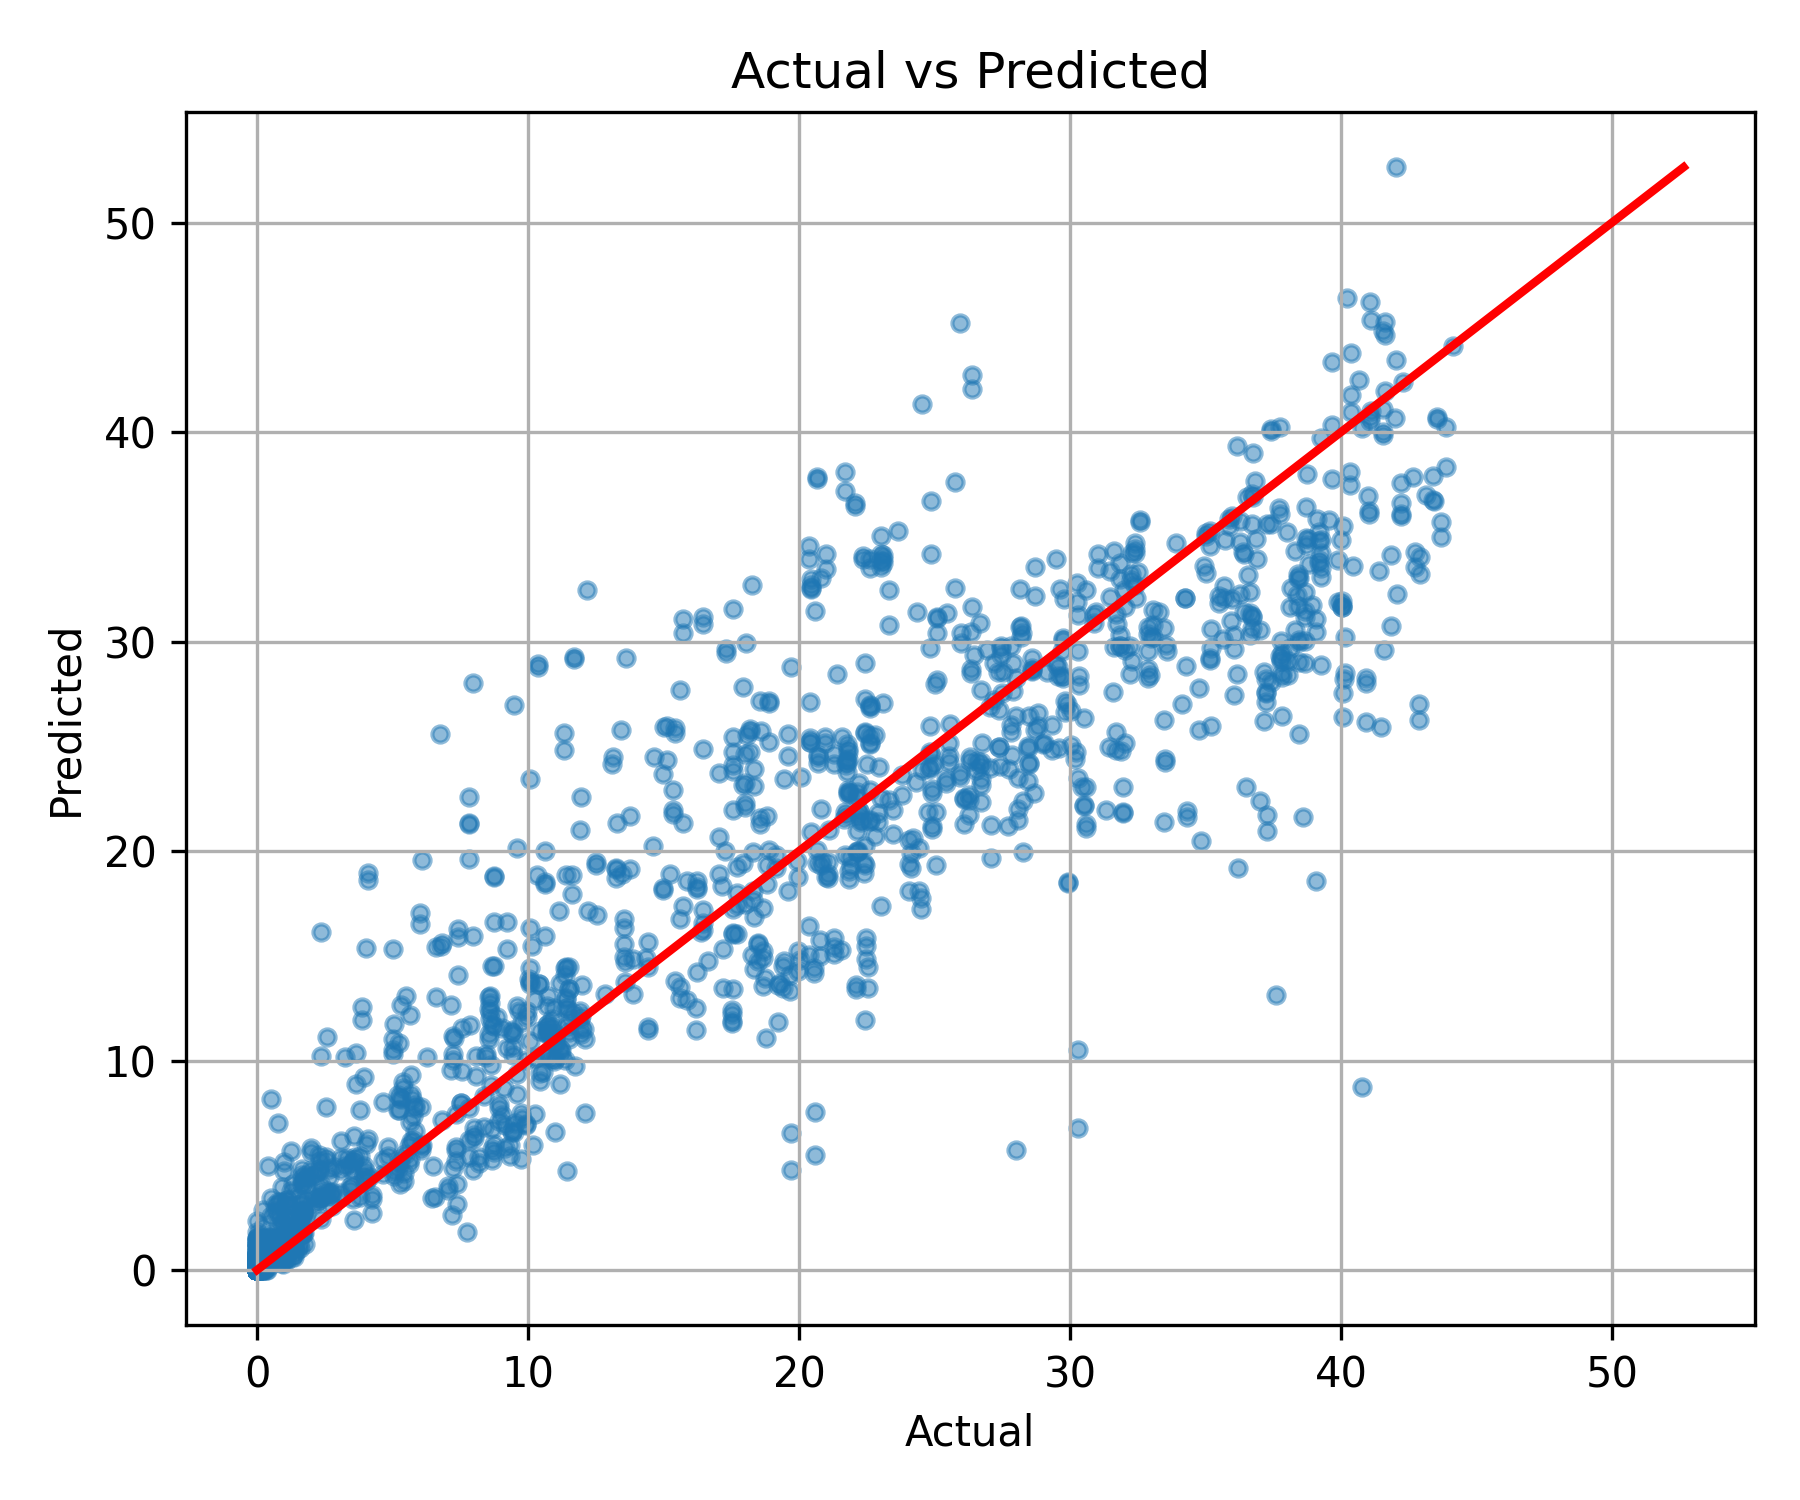
\includegraphics[width=0.7\textwidth]{picture/2_actual_vs_predicted.png}
    \caption[กราฟ Actual vs Predicted]{กราฟ Actual vs Predicted}
    \label{fig:image1}
\end{figure}

\vspace{10pt}
\begin{flushleft}
\hspace*{0.5cm}
จากกราฟเปรียบเทียบค่า Actual และ Prediction โดยแกน x คือ Actual และ แกน y คือ Prediction โดยพบว่าค่าการทำนายมีความสอดคล้องกับค่าจริงในภาพรวม โดยจุดข้อมูลส่วนใหญ่กระจายตัวใกล้กับเส้นทแยงมุมสีแดง แสดงให้เห็นว่าโมเดลสามารถเรียนรู้ความสัมพันธ์ระหว่างตัวแปรสภาพอากาศกับการผลิตไฟฟ้าจากโซลาร์เซลล์ได้อย่างมีประสิทธิภาพ 
อย่างไรก็ตาม ในช่วงค่าการผลิตไฟฟ้าสูง จะพบการกระจายตัวของจุดข้อมูลเพิ่มขึ้น ซึ่งสะท้อนให้เห็นว่าความคลาดเคลื่อนของโมเดลมีแนวโน้มเพิ่มขึ้นเมื่อกำลังผลิตสูงขึ้น อาจเกิดจากความผันผวนของสภาพอากาศแบบฉับพลัน เช่น เมฆบังแดด หรือการเปลี่ยนแปลงของอุณหภูมิที่รวดเร็ว
\end{flushleft}



\subsection{การวิเคราะห์ Residual Plot}

\begin{figure}[H]
    \centering
    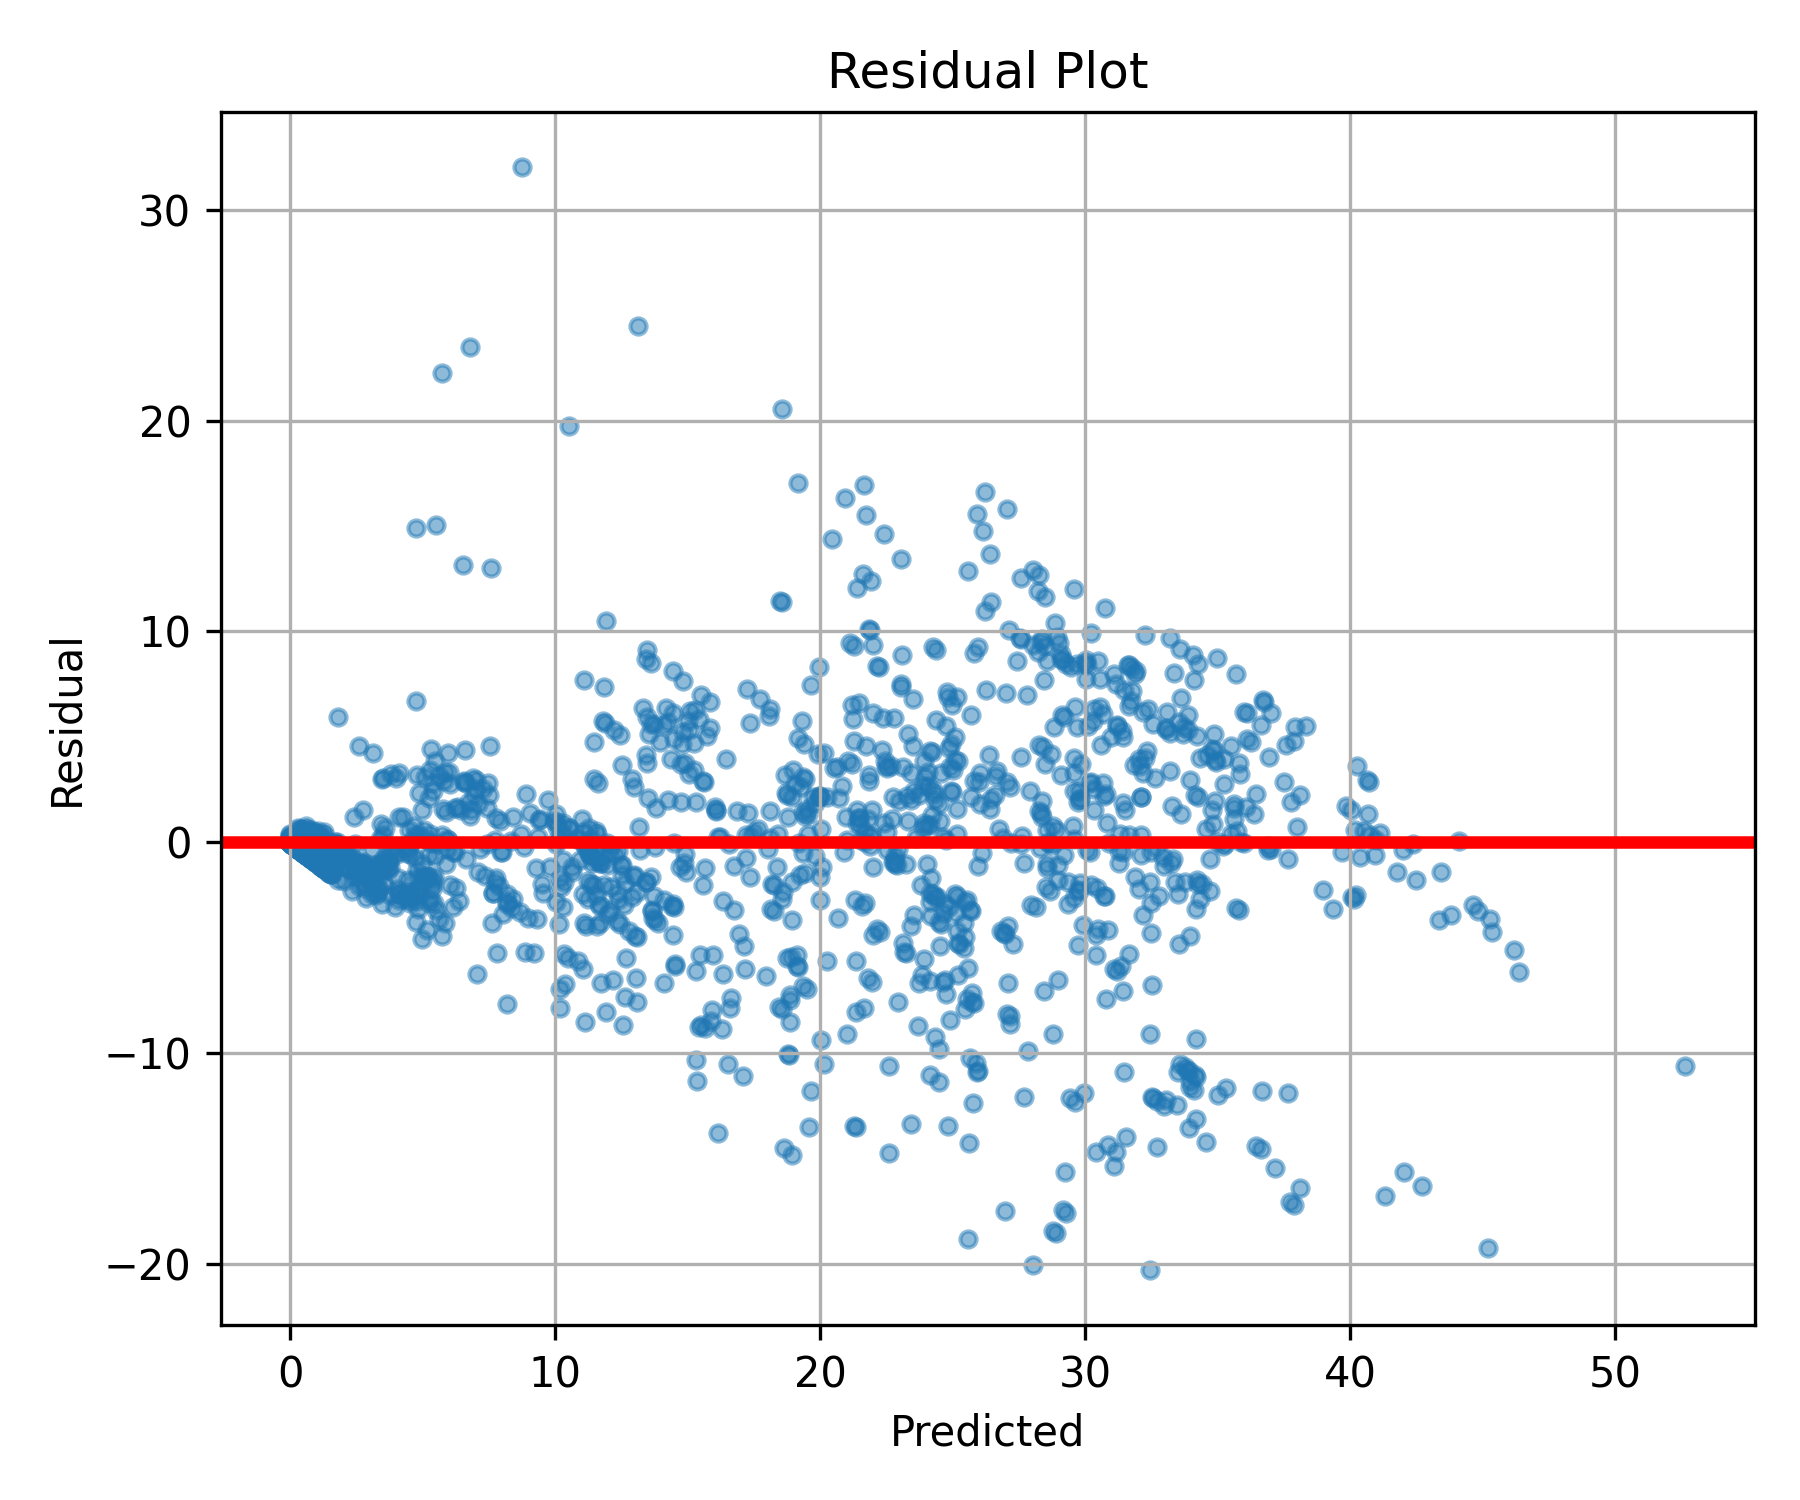
\includegraphics[width=0.7\textwidth]{picture/3_residual_plot.png}
    \caption[Residual Plot]{Residual Plot}
    \label{fig:image2}
\end{figure}

\vspace{10pt}
\begin{flushleft}
\hspace*{0.5cm}
จากกราฟจะพบว่าค่าความคลาดเคลื่อนส่วนใหญ่กระจายอยู่รอบค่า 0 แสดงว่าโมเดลไม่มีแนวโน้มทำนายค่าสูงเกินจริง หรือ ต่ำเกินจริง อย่างไรก็ตาม จะเห็นว่าการกระจายของ residual มีลักษณะขยายตัวมากขึ้นเมื่อค่าที่ทำนายมีค่าสูง ซึ่งแสดงถึงความแปรปรวนของความคลาดเคลื่อนที่เพิ่มขึ้นตามระดับกำลังผลิตไฟฟ้า 
อาจเป็นผลมาจากปัจจัยภายนอกที่มีผลต่อการผลิตไฟฟ้าในช่วงเวลานั้น เช่น สภาพอากาศที่ไม่คงที่ หรือข้อจำกัดของชุดข้อมูลในการฝึกฝนโมเดล
\end{flushleft}



\subsection{การวิเคราะห์ Feature Importance}

\begin{figure}[H]
    \centering
    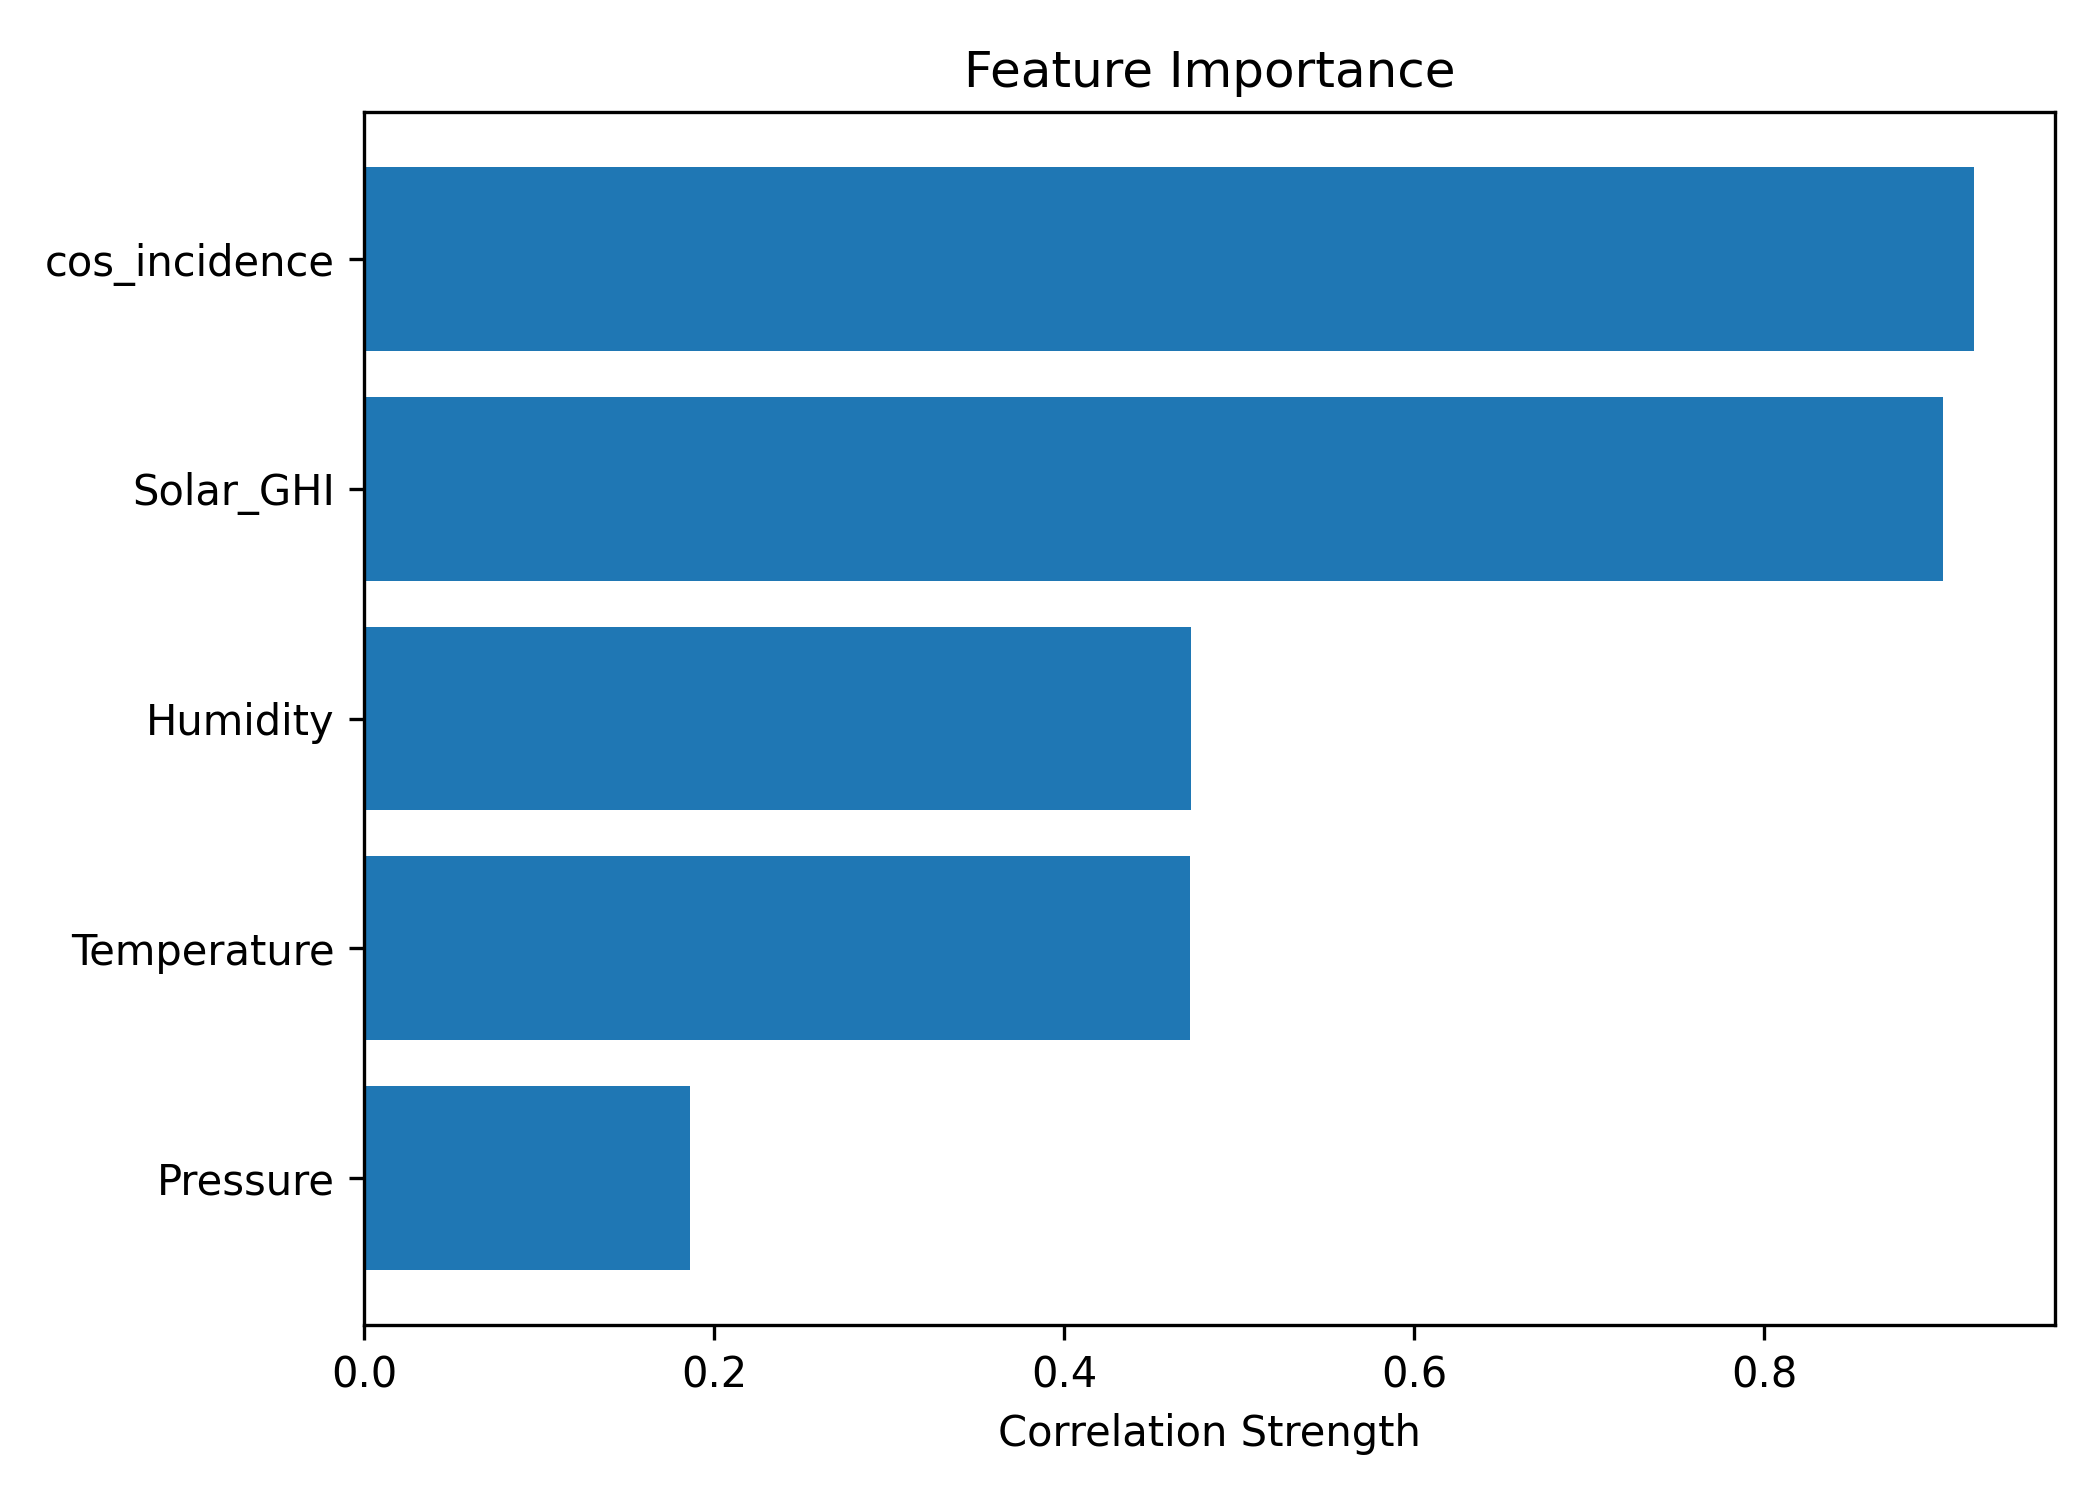
\includegraphics[width=0.7\textwidth]{picture/5_feature_importance.png}
    \caption[Feature Importance]{Feature Importance}
    \label{fig:image3}
\end{figure}

\vspace{10pt}
\begin{flushleft}
\hspace*{0.5cm}
จากรูปจะเห็นได้ว่าค่ามุมตกกระทบของแสงกับแผงโซลาร์เซลล์ (cos\_incidence) เป็นตัวแปรที่มีความสำคัญมากที่สุดรองลงมาก็คือ ความเข้มแสง (Solar\_GHI) ต่อมาคือความชื้นและอุณหภูมิ มีความสำคัญในระดับปานกลาง และสุดท้ายที่ส่งผลต่อโมเดลน้อยที่สุดคือ ความกดอากาศ
\end{flushleft}


\section{การทำงานของ Web Dashboard}

\subsection{หน้าแรก}

\begin{figure}[H]
    \centering
    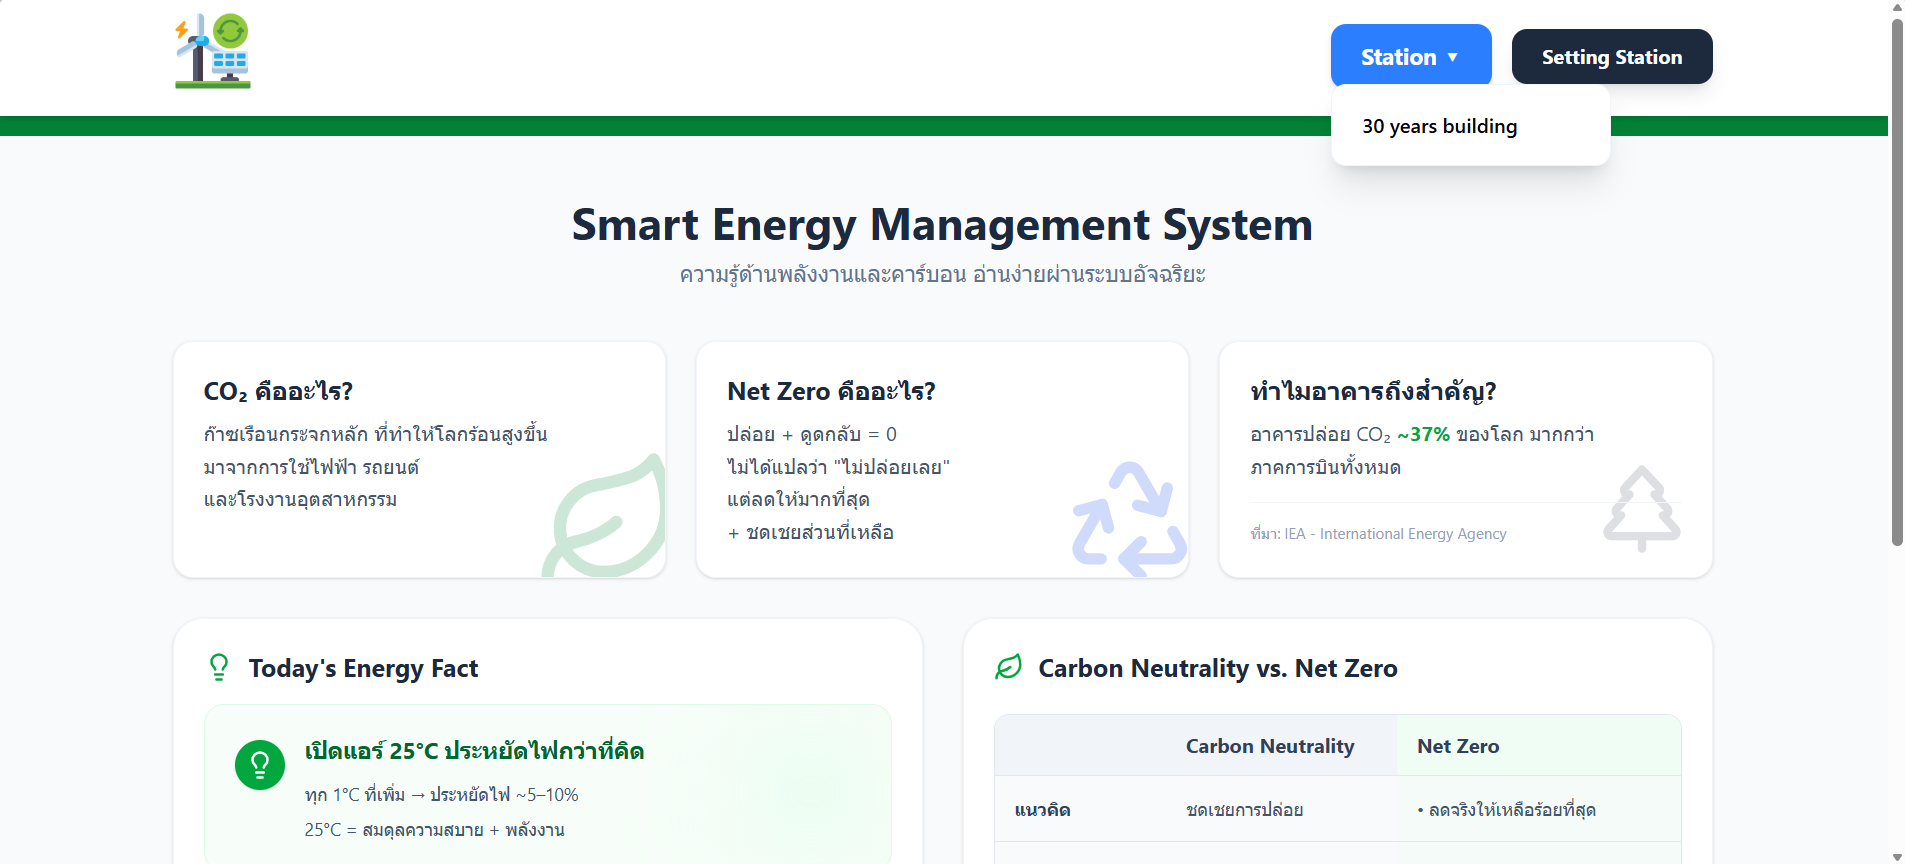
\includegraphics[width=0.7 \textwidth]{picture/Home.png}
    \caption[หน้าแรก]{หน้าแรก}
    \label{fig:image4}
\end{figure}

\vspace{10pt}
\begin{itemize}
    \item[]\textbf{4.3.1 ผลการประเมินเชิงตัวเลข} ค่าประสิทธิภาพของโมเดลมีดังนี้
    \begin{itemize}
        \item $R^2$ = 0.8619
        \item MAE = 2.427 kWh
    \end{itemize}

    \item[]\textbf{4.3.2 กราฟ Actual vs Predicted} 
    
    \hspace{\parindent} จากกราฟเปรียบเทียบค่า Actual และ Prediction โดยแกน x คือ Actual และ แกน y คือ Prediction โดยพบว่าค่าการทำนายมีความสอดคล้องกับค่าจริงในภาพรวม โดยจุดข้อมูลส่วนใหญ่กระจายตัวใกล้กับเส้นทแยงมุมสีแดง แสดงให้เห็นว่าโมเดลสามารถเรียนรู้ความสัมพันธ์ระหว่างตัวแปรสภาพอากาศกับการผลิตไฟฟ้าจากโซลาร์เซลล์ได้อย่างมีประสิทธิภาพ อย่างไรก็ตาม ในช่วงค่าการผลิตไฟฟ้าสูง จะพบการกระจายตัวของจุดข้อมูลเพิ่มขึ้น ซึ่งสะท้อนให้เห็นว่าความคลาดเคลื่อนของโมเดลมีแนวโน้มเพิ่มขึ้นเมื่อกำลังผลิตสูงขึ้น อาจเกิดจากความผันผวนของสภาพอากาศแบบฉับพลัน เช่น เมฆบังแดด หรือการเปลี่ยนแปลงของอุณหภูมิที่รวดเร็ว
    
    \begin{figure}[H]
    \centering
    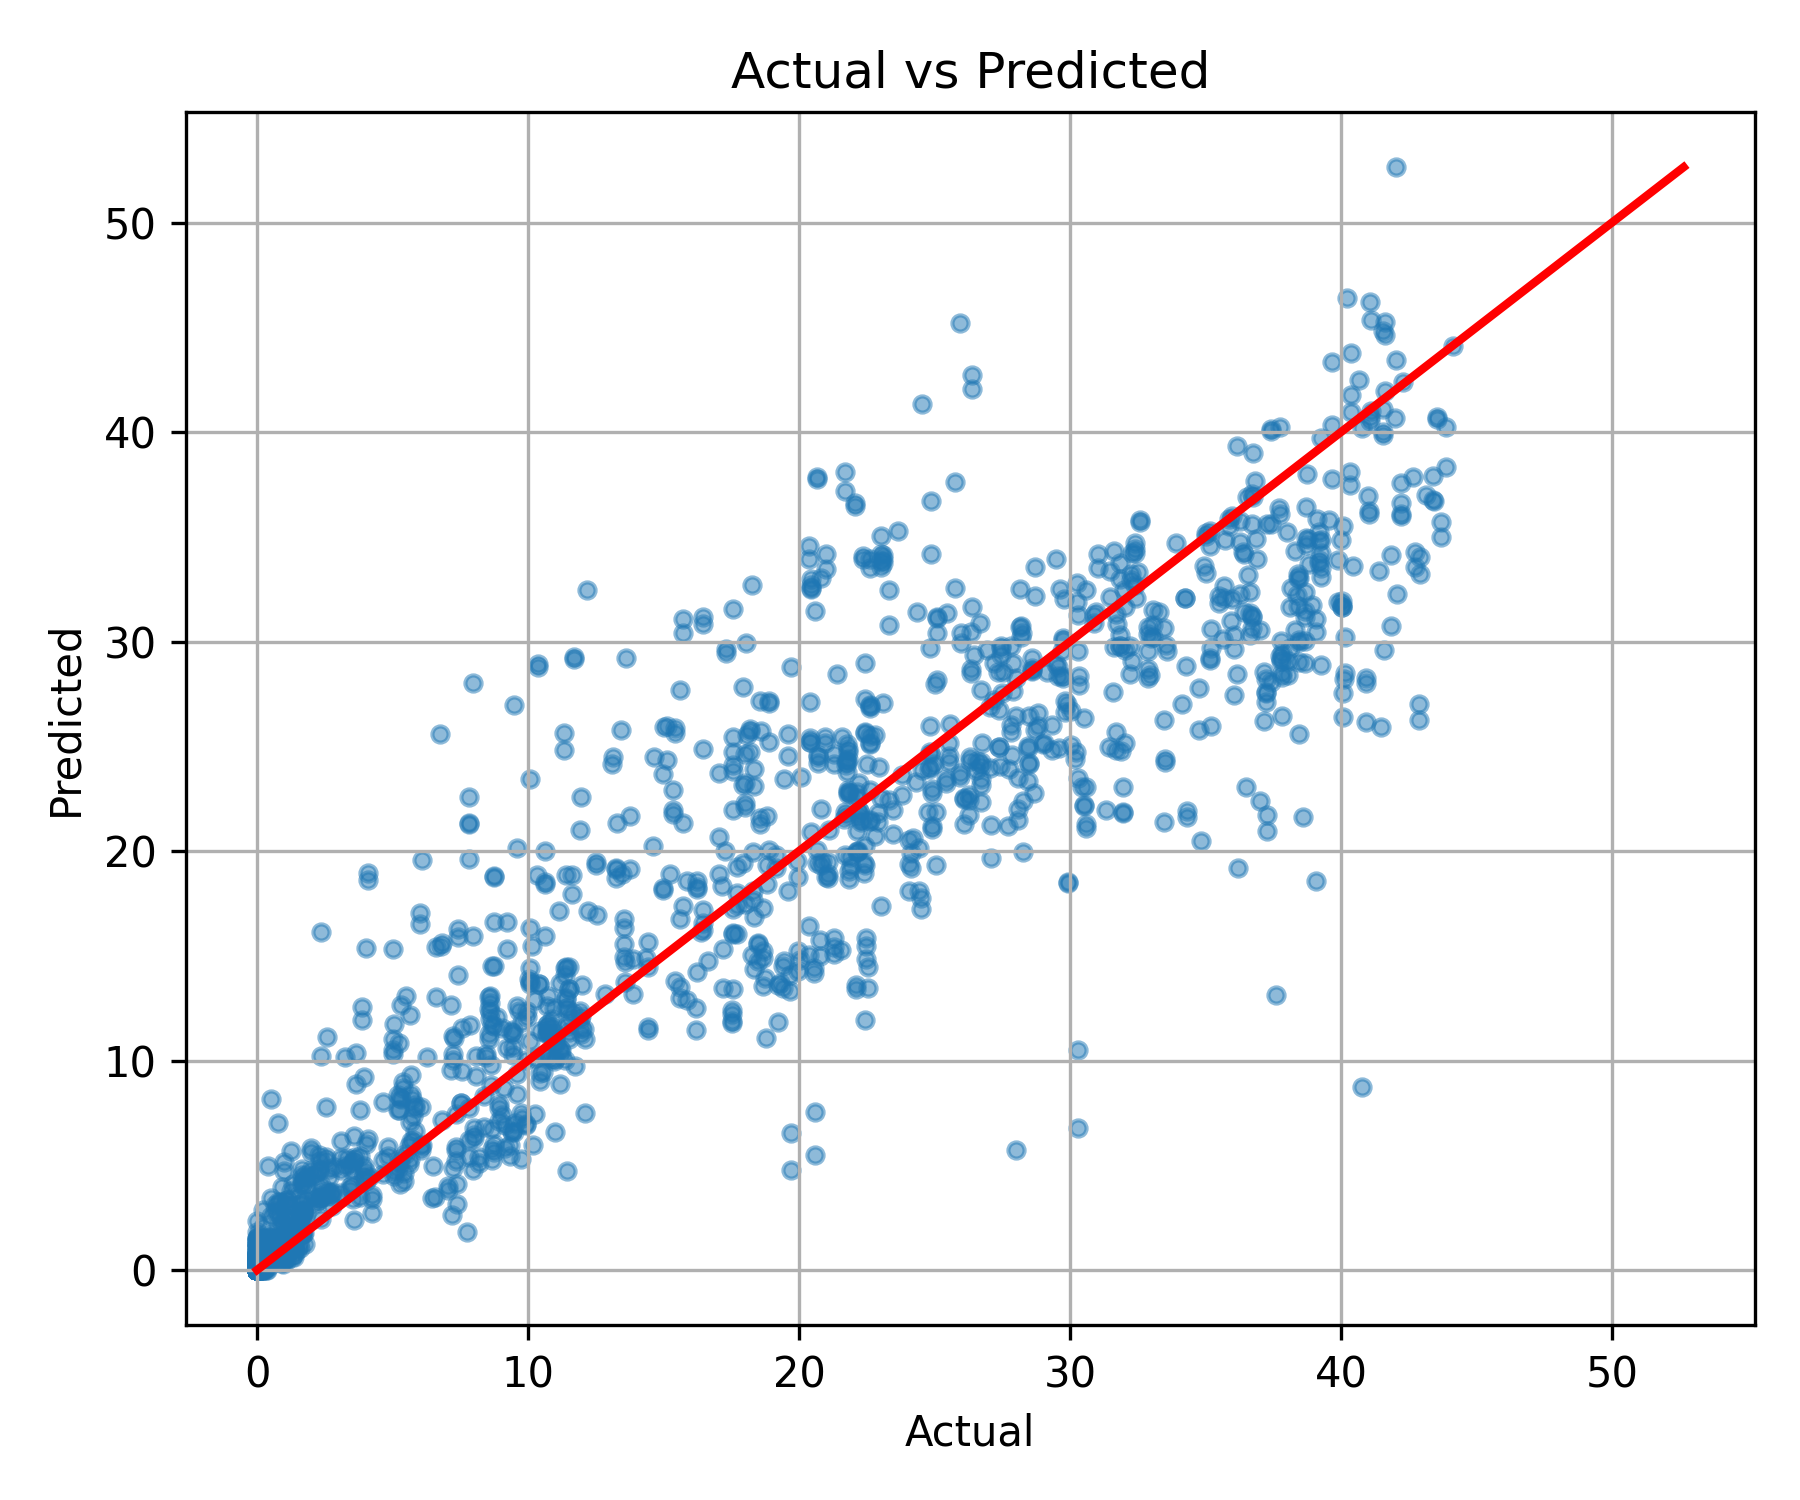
\includegraphics[width=0.7\textwidth]{picture/2_actual_vs_predicted.png}
    \caption[กราฟ Actual vs Predicted]{กราฟ Actual vs Predicted}
    \label{fig:Actual vs Predicted}
    \end{figure}
 
    \item[]\textbf{4.3.3 กราฟ Residual Plot} 
    
    \hspace{\parindent} จากกราฟจะพบว่าค่าความคลาดเคลื่อนส่วนใหญ่กระจายอยู่รอบค่า 0 แสดงว่าโมเดลไม่มีแนวโน้มทำนายค่าสูงเกินจริง หรือ ต่ำเกินจริง อย่างไรก็ตาม จะเห็นว่าการกระจายของ residual มีลักษณะขยายตัวมากขึ้นเมื่อค่าที่ทำนายมีค่าสูง ซึ่งแสดงถึงความแปรปรวนของความคลาดเคลื่อนที่เพิ่มขึ้นตามระดับกำลังผลิตไฟฟ้า 
    อาจเป็นผลมาจากปัจจัยภายนอกที่มีผลต่อการผลิตไฟฟ้าในช่วงเวลานั้น เช่น สภาพอากาศที่ไม่คงที่ หรือข้อจำกัดของชุดข้อมูลในการฝึกฝนโมเดล
   
    \begin{figure}[H]
    \centering
    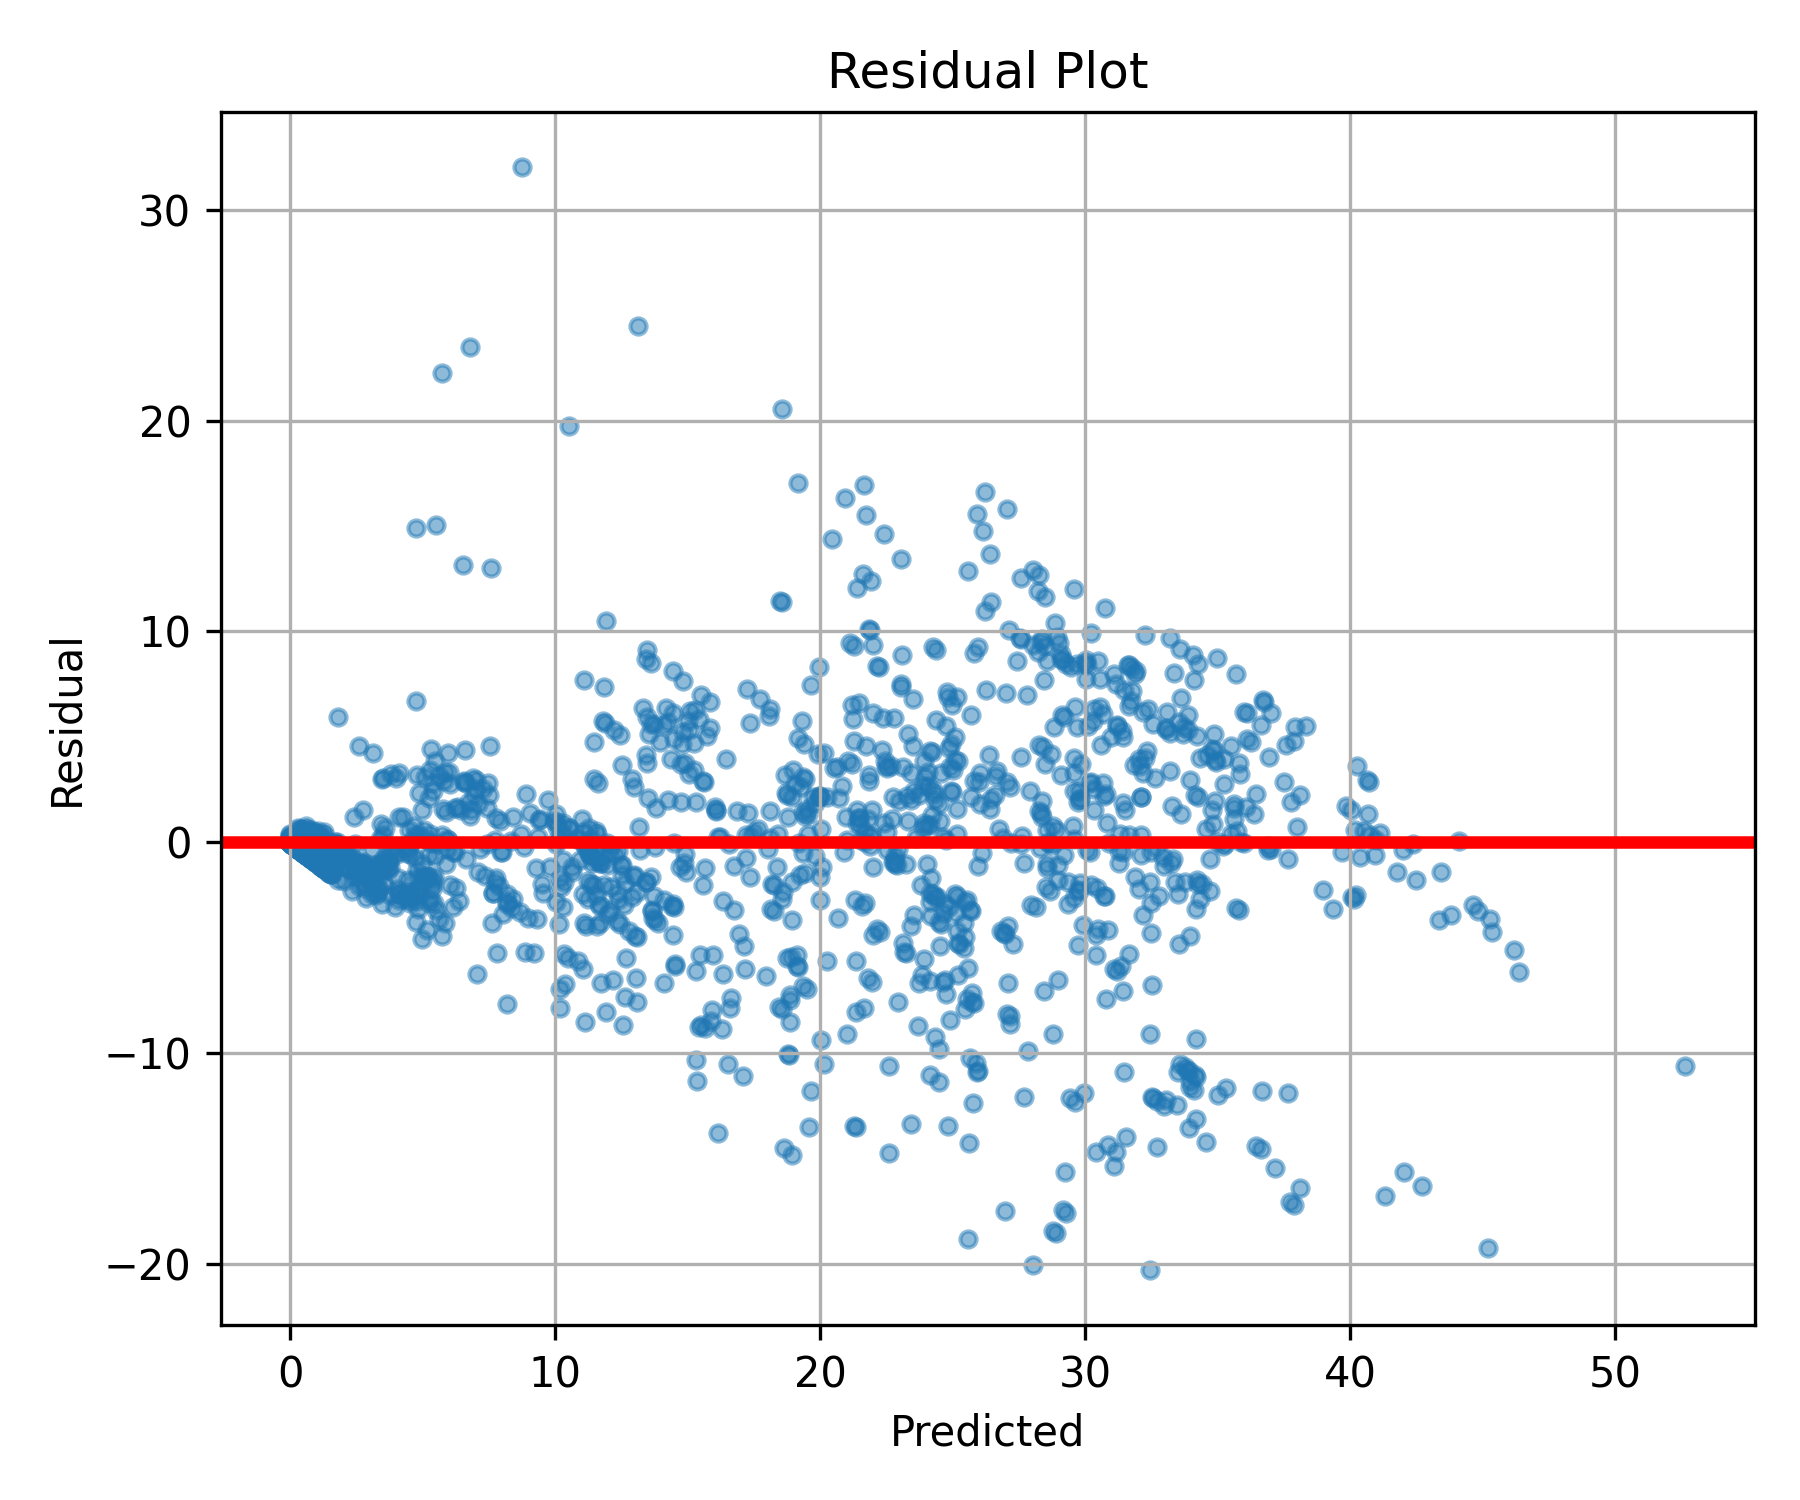
\includegraphics[width=0.7\textwidth]{picture/3_residual_plot.png}
    \caption[Residual Plot]{Residual Plot}
    \label{fig:Residual Plot}
    \end{figure}
   
    \item[] \textbf{4.3.4 กราฟ Feature Importance} 
    \hspace{\parindent} จากรูปจะเห็นได้ว่าค่ามุมตกกระทบของแสงกับแผงโซลาร์เซลล์ (cos\_incidence) เป็นตัวแปรที่มีความสำคัญมากที่สุดรองลงมาก็คือ ความเข้มแสง (Solar\_GHI) ต่อมาคือความชื้นและอุณหภูมิ มีความสำคัญในระดับปานกลาง และสุดท้ายที่ส่งผลต่อโมเดลน้อยที่สุดคือ ความกดอากาศ
    \begin{figure}[H]
    \centering
    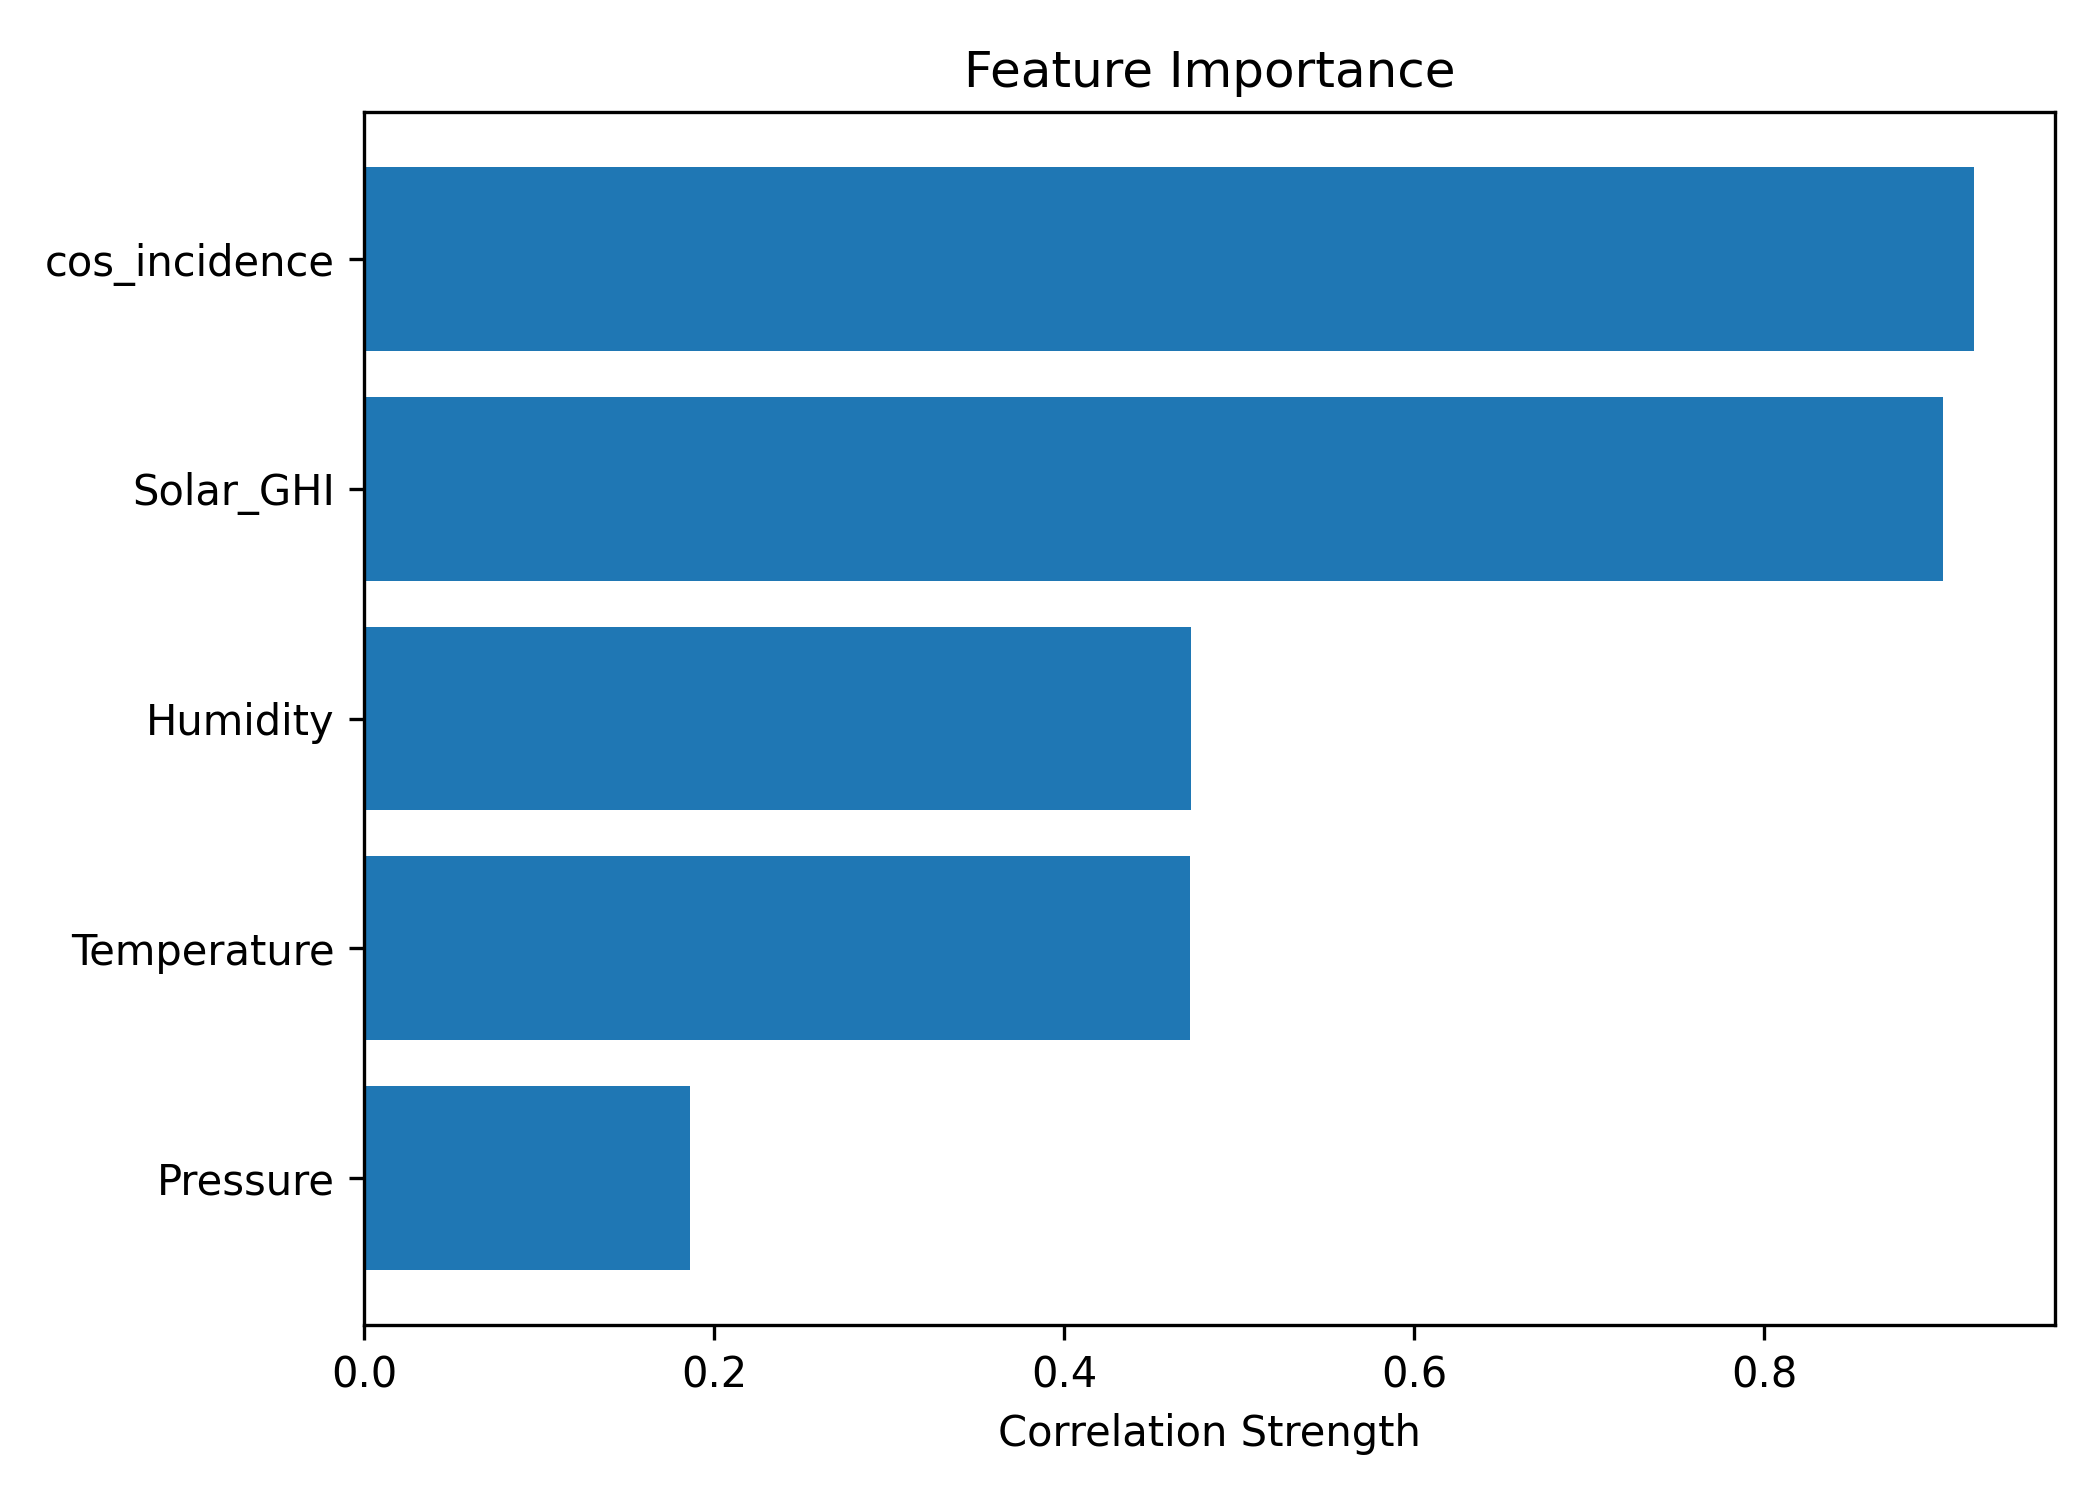
\includegraphics[width=0.7\textwidth]{picture/5_feature_importance.png}
    \caption[Feature Importance]{Feature Importance}
    \label{fig:Feature Importance}
    \end{figure}

\end{itemize}

\section{การใช้งานทั้งระบบ}
\begin{itemize}
    \item[]\textbf{4.4.1 การทดสอบการใช้งานระบบ} 
    \hspace{\parindent} ได้ทำการทดสอบการใช้งานระบบโดยการติดตั้งสถานีวัดสภาพอากาศขนาดย่อมที่บริเวณหลังคาของอาคาร ตึก 30 ปีคณะวิศวกรรมศาสตร์ มหาวิทยาลัยเชียงใหม่ และทำการทดสอบระบบโดยการให้ผู้ทดลองใช้งานระบบเพื่อดูข้อมูลสภาพอากาศและข้อมูลการพยากรณ์ปริมาณการผลิตไฟฟ้าจากโซลาร์เซลล์ล่วงหน้า 24 ชั่วโมง เป็นเวลา 10 วัน โดยผลการทดสอบพบว่ามีค่าความคลาดเคลื่อนเฉลี่ย 4.574 kWhต่อจุดข้อมูล ซึ่งเป็นผลมาจากความแปรปรวนของสภาพอากาศ และ ข้อจำกัดของชุดข้อมูลที่ใช้ในการฝึกฝนโมเดล เนื่องจากข้อมูลสภาพอากาศที่นำมาฝึกฝนโมเดลไม่ได้ใช้ค่าที่มาจากสถานีวัดสภาพอากาศที่ทำขึ้นแต่ตอนทดสอบใช้สภาพอากาศจากสถานีในการทำการทดสอบ จึงทำให้ค่าที่ทำนายการผลิตไฟฟ้านั้นเกิดความคลาดเคลื่อน 

    \begin{figure}[H]
    \centering
    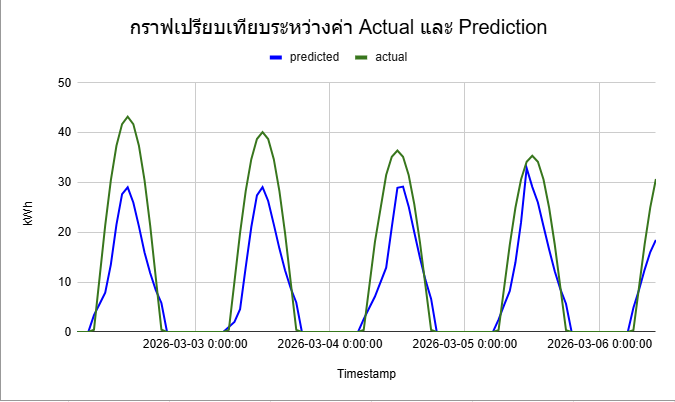
\includegraphics[width=0.7\textwidth]{picture/Test Station.png}
    \caption[การทดสอบการใช้งานระบบ]{การทดสอบการใช้งานระบบ}
    \label{fig:Test Station}
    \end{figure}

    \item[]\textbf{4.4.2 การประเมินความพึงพอใจในการใช้งานระบบ} 
    \hspace{\parindent} ได้ทําการประเมินความพึงพอใจในการใช้งานระบบ โดยมีนักศึกษามหาวิทยาลัยเชียงใหม่ 21 คนทําการประเมินโดยแบ่งเป็นผู้ชาย 10 คน และผู้หญิง 11 คน โดยให้คะแนนในแต่ละหัวข้อการประเมินตามความพึงพอใจในการใช้งานระบบ ซึ่งผลการประเมินมีดังนี้
    \begin{table}[H]
    \centering
    \renewcommand{\arraystretch}{1.5}
    \begin{tabular}{|l|c|}
    \hline 
    \multicolumn{1}{|c|}{\textbf{หัวข้อการประเมิน}} & \textbf{ความพึงพอใจ(เต็ม 5 คะแนน)} \\ \hline
    ด้านการออกแบบเว็บไซต์ (Interface Design) & 4.84 \\ \hline
    ด้านการแสดงผลข้อมูล (Data Visualization)   & 4.72 \\ \hline
    ด้านการใช้งานระบบ (Usability)   & 4.71 \\ \hline
    ด้านประสิทธิภาพของระบบ (System Performance)   & 4.67  \\ \hline
    ด้านประโยชน์ของระบบ (Usefulness) & 4.84  \\ \hline
    การเข้าถึงระบบ (Accessibility) & 4.80  \\ \hline
    \end{tabular}
    \caption{ประเมินความพึงพอใจในการใช้งานระบบ}
    \label{tab:satisfaction}
    \end{table}
    \vspace{10pt}
    \begin{flushleft}
    \hspace*{0.5cm}
    จากผลการประเมินความพึงพอใจรวมของผู้ทดลองใช้เว็บไซต์คือ 4.77 คะแนนหรือคิดเป็น 95.34\%
    \end{flushleft}
\end{itemize}


\section{วิเคราะห์และอภิปรายผล}
\hspace{\parindent} จากการใช้งานระบบพยากรณ์ปริมาณการผลิตไฟฟ้าจากแผงโซลาร์เซลล์ ซึ่งประกอบด้วยสถานีวัดสภาพอากาศขนาดย่อม Web Dashboard และ โมเดล Machine Learning สามารถวิเคราะห์และอภิปรายผลได้ดังนี้

\begin{figure}[H]
\centering
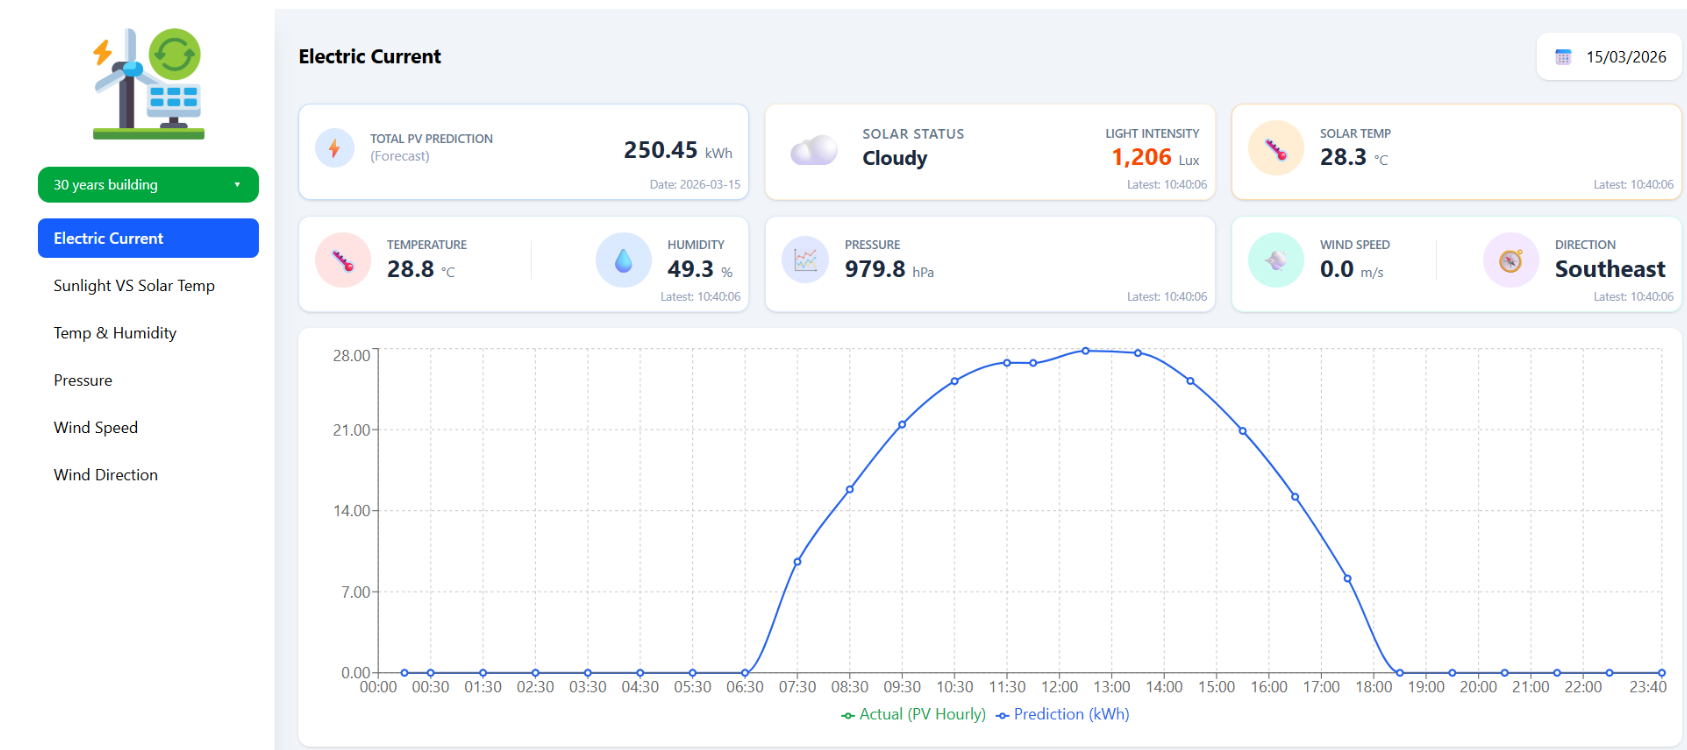
\includegraphics[width=0.7\textwidth]{picture/prediction.png}
\caption[หน้าแสดงข้อมูลการพยากรณ์ปริมาณการผลิตไฟฟ้าจากแผงโซลาร์เซลล์]{หน้าแสดงข้อมูลการพยากรณ์ปริมาณการผลิตไฟฟ้าจากแผงโซลาร์เซลล์}
\label{fig:image5}
\end{figure}

\vspace{10pt}
\begin{itemize}
    \item แสดงผลรวมการพยากร์ณปริมาณการผลิตไฟฟ้าจากโซลาร์เซลล์
    \item แสดงข้อมูลสภาพอากาศล่าสุดที่วัดได้จากเซ็นเซอร์
    \item แสดงกราฟการผลิตไฟฟ้าแบบรายชั่วโมงที่พยากรณ์ไว้ล่วงหน้า
\end{itemize}

\subsection{หน้าแสดงข้อมูลปริมาณไฟฟ้าที่ผลิตได้จริงจากแผงโซลลาร์เซลล์}

\begin{figure}[H]
\centering
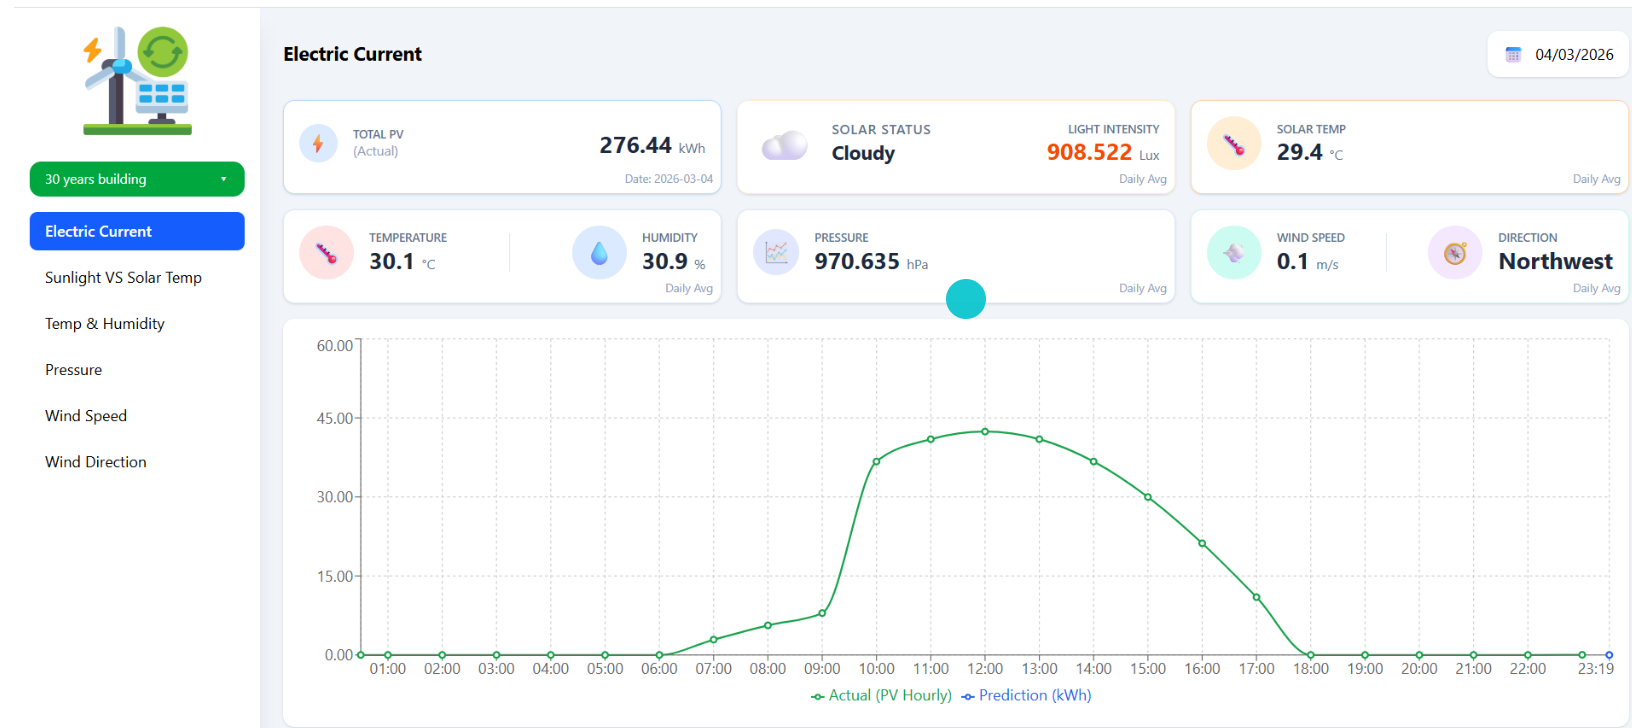
\includegraphics[width=0.7\textwidth]{picture/Electric Current.png}
\caption[หน้าแสดงข้อมูลปริมาณไฟฟ้าที่ผลิตได้จริงจากแผงโซลลาร์เซลล์]{หน้าแสดงข้อมูลปริมาณไฟฟ้าที่ผลิตได้จริงจากแผงโซลลาร์เซลล์}
\label{fig:image6}
\end{figure}
\vspace{10pt}

\begin{itemize}
    \item แสดงผลรวมปริมาณการผลิตไฟฟ้าจากโซลาร์เซลล์ที่ได้ในแต่ละวัน
    \item แสดงข้อมูลสภาพอากาศภาพเฉลี่ยรายวันที่วัดได้จากเซ็นเซอร์
    \item แสดงกราฟปริมาณการผลิตไฟฟ้าที่เกิดขึ้นจริงแบบรายชั่วโมง
    \item ผู้ใช้สามารถเลือกดูข้อมูลย้อนหลังหรือล่วงหน้าได้ผ่านปฏิทินที่มุมขวาบน 
    \item ผู้ใช้สามารถเลือกดูข้อมูลของแต่ละอาคารได้จากเมนูด้านซ้าย
\end{itemize}

\subsection{หน้าแสดงข้อมูลปริมาณแสงอาทิตย์และอุณหภูมิแผงโซลลาร์เซลล์}

\begin{figure}[H]
\centering
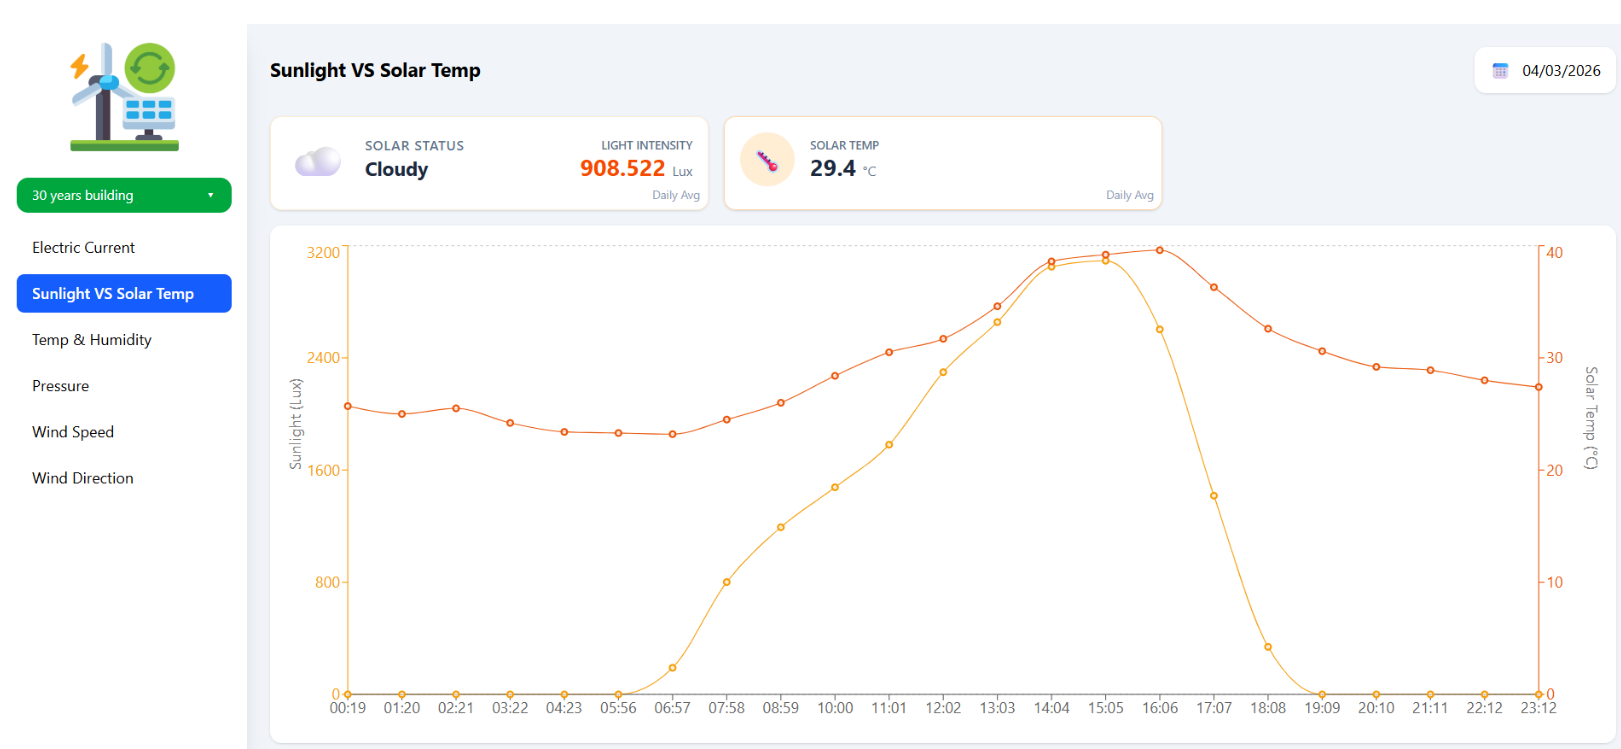
\includegraphics[width=0.7\textwidth]{picture/Sunlight VS Solar Temp.png}
\caption[หน้าแสดงข้อมูลปริมาณแสงอาทิตย์และอุณหภูมิแผงโซลลาร์เซลล์]{หน้าแสดงข้อมูลปริมาณแสงอาทิตย์และอุณหภูมิแผงโซลลาร์เซลล์}
\label{fig:image7}
\end{figure}

\vspace{10pt}
\begin{itemize}
    \item แสดงกราฟเปรียบเทียบระหว่างความเข้มแสงและอุณหภูมิแผงโซลลาร์เซลล์
    \item แสดงข้อมูลความเข้มแสงและอุณหภูมิแผงโซลลาร์เซลล์เฉลี่ยรายวัน 
    \item แสดงให้เห็นถึงความสัมพันธ์และแนวโน้มของอุณหภูมิแผงโซลาร์เซลล์ที่แปรผันตามความเข้มของแสงแดดในแต่ละช่วงเวลาของวัน
\end{itemize}

\subsection{หน้าแสดงข้อมูลอุณหภูมิและความชื้น}

\begin{figure}[H]
\centering
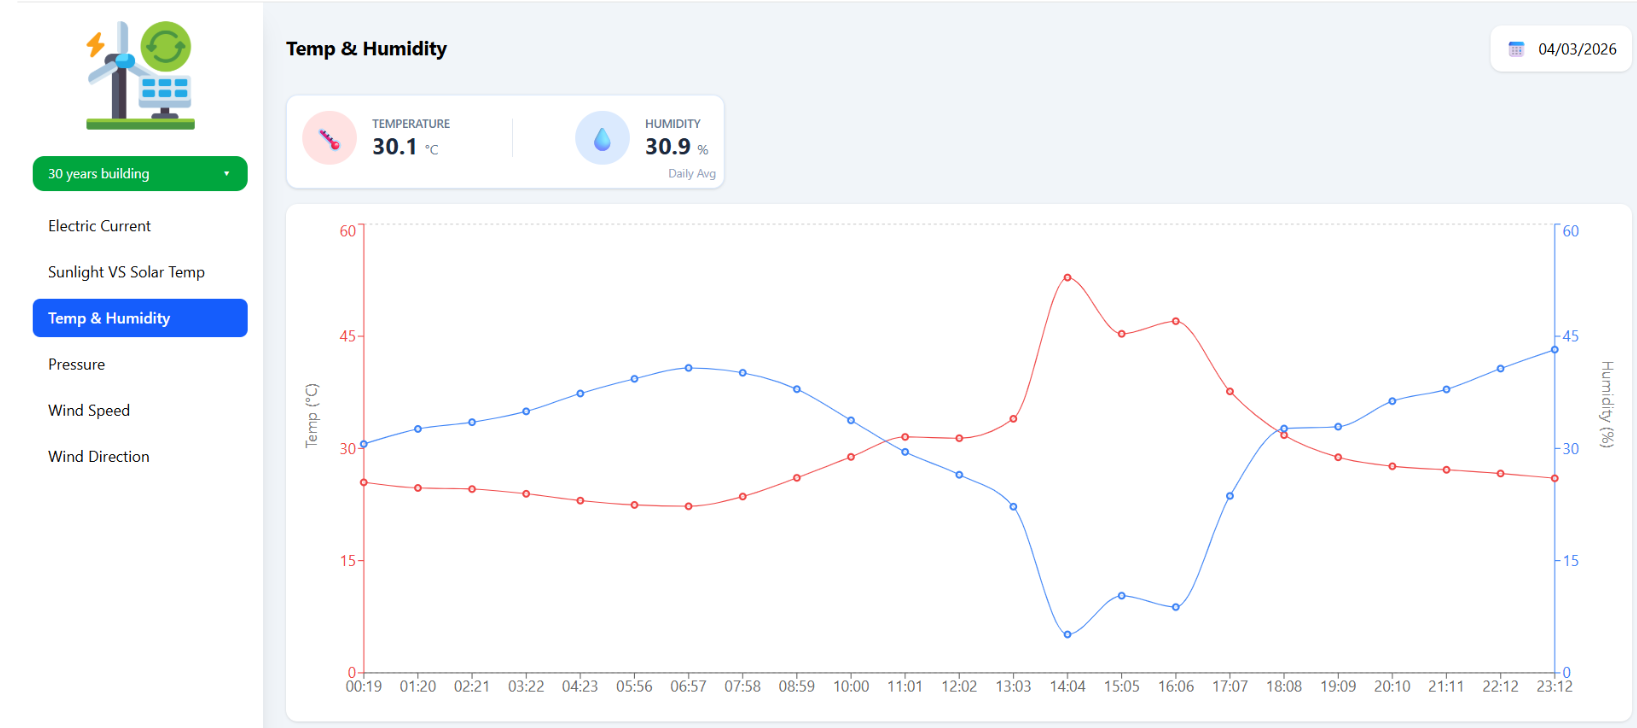
\includegraphics[width=0.7\textwidth]{picture/Temp and Humidity.png}
\caption[หน้าแสดงข้อมูลอุณหภูมิและความชื้น]{หน้าแสดงข้อมูลอุณหภูมิและความชื้น}
\label{fig:image8}
\end{figure}

\vspace{10pt}
\begin{itemize}
    \item แสดงกราฟเปรียบเทียบระหว่างอุณหภูมิและความชื้น
    \item แสดงข้อมูลอุณหภูมิและความชื้นเฉลี่ยรายวัน 
\end{itemize}



\subsection{หน้าแสดงข้อมูลความกดอากาศ}

\begin{figure}[H]
\centering
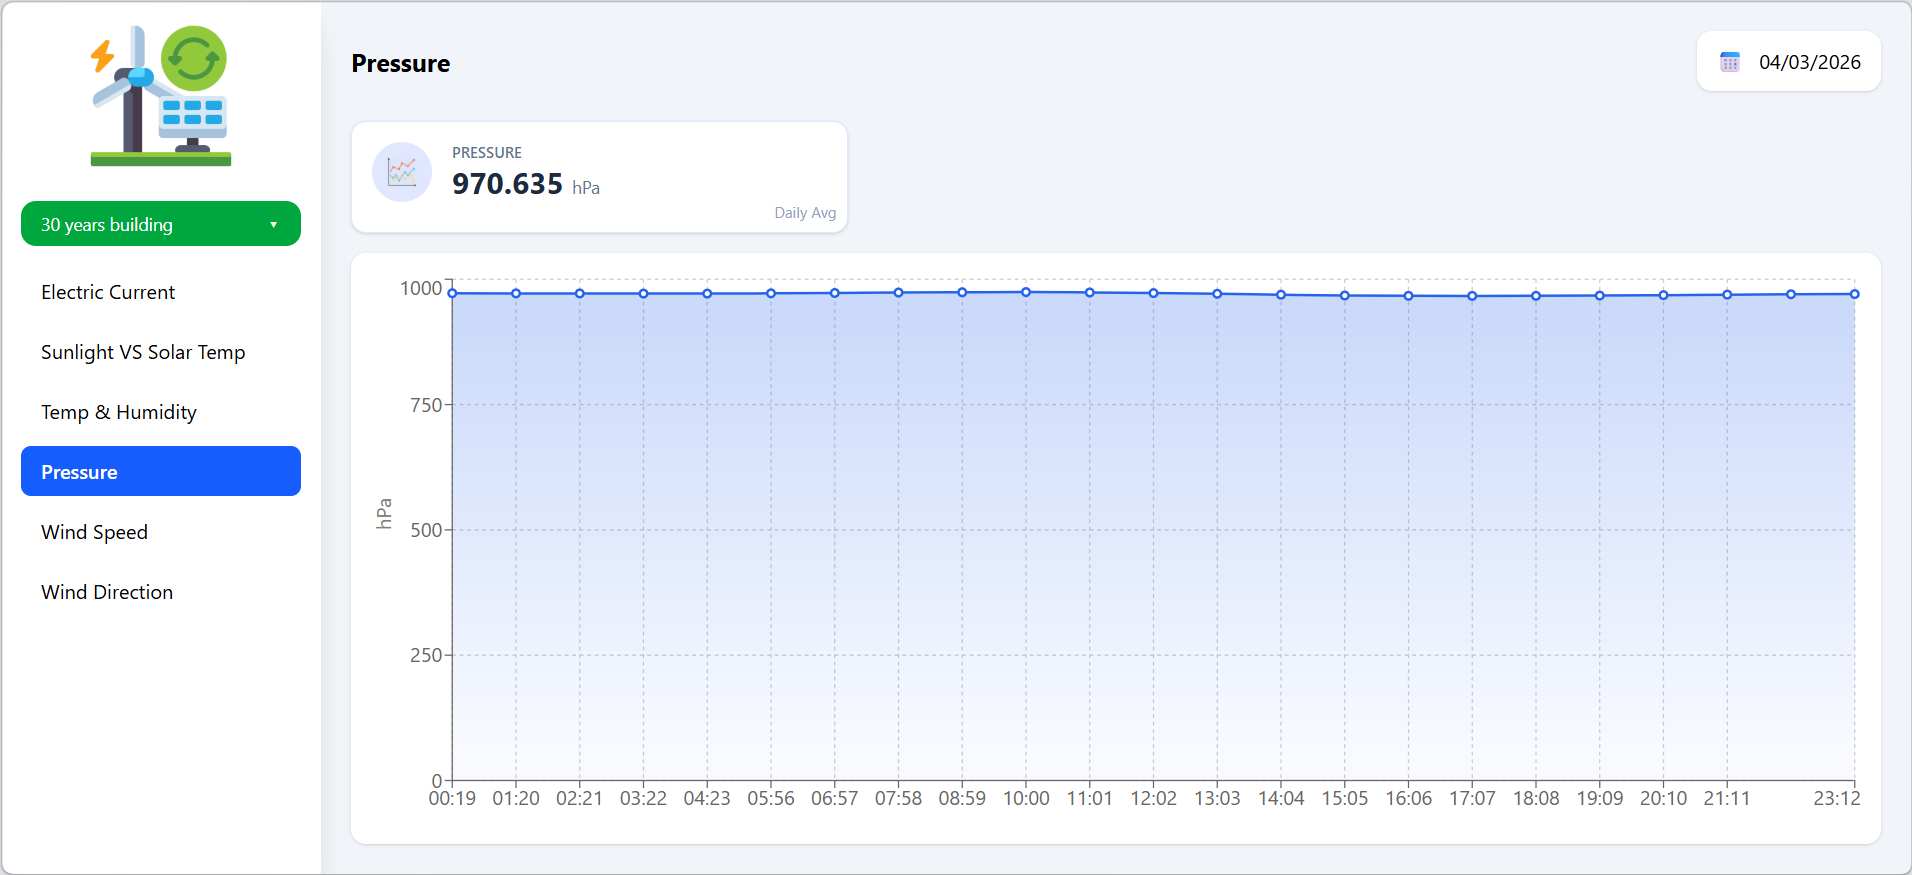
\includegraphics[width=0.7\textwidth]{picture/Pressure.png}
\caption[หน้าแสดงข้อมูลความกดอากาศ]{หน้าแสดงข้อมูลความกดอากาศ}
\label{fig:image9}
\end{figure}

\vspace{10pt}
\begin{itemize}
    \item แสดงข้อมูลความกดอากาศเฉลี่ยรายวัน 
    \item แสดงกราฟความกดอากาศในแต่ละช่วงเวลาของวัน เพื่อใช้เป็นข้อมูลประกอบในการวิเคราะห์การเกิดฝนตกหรือมีเมฆมาก
\end{itemize}

\subsection{หน้าแสดงข้อมูลความเร็วลม}

\begin{figure}[H]
\centering
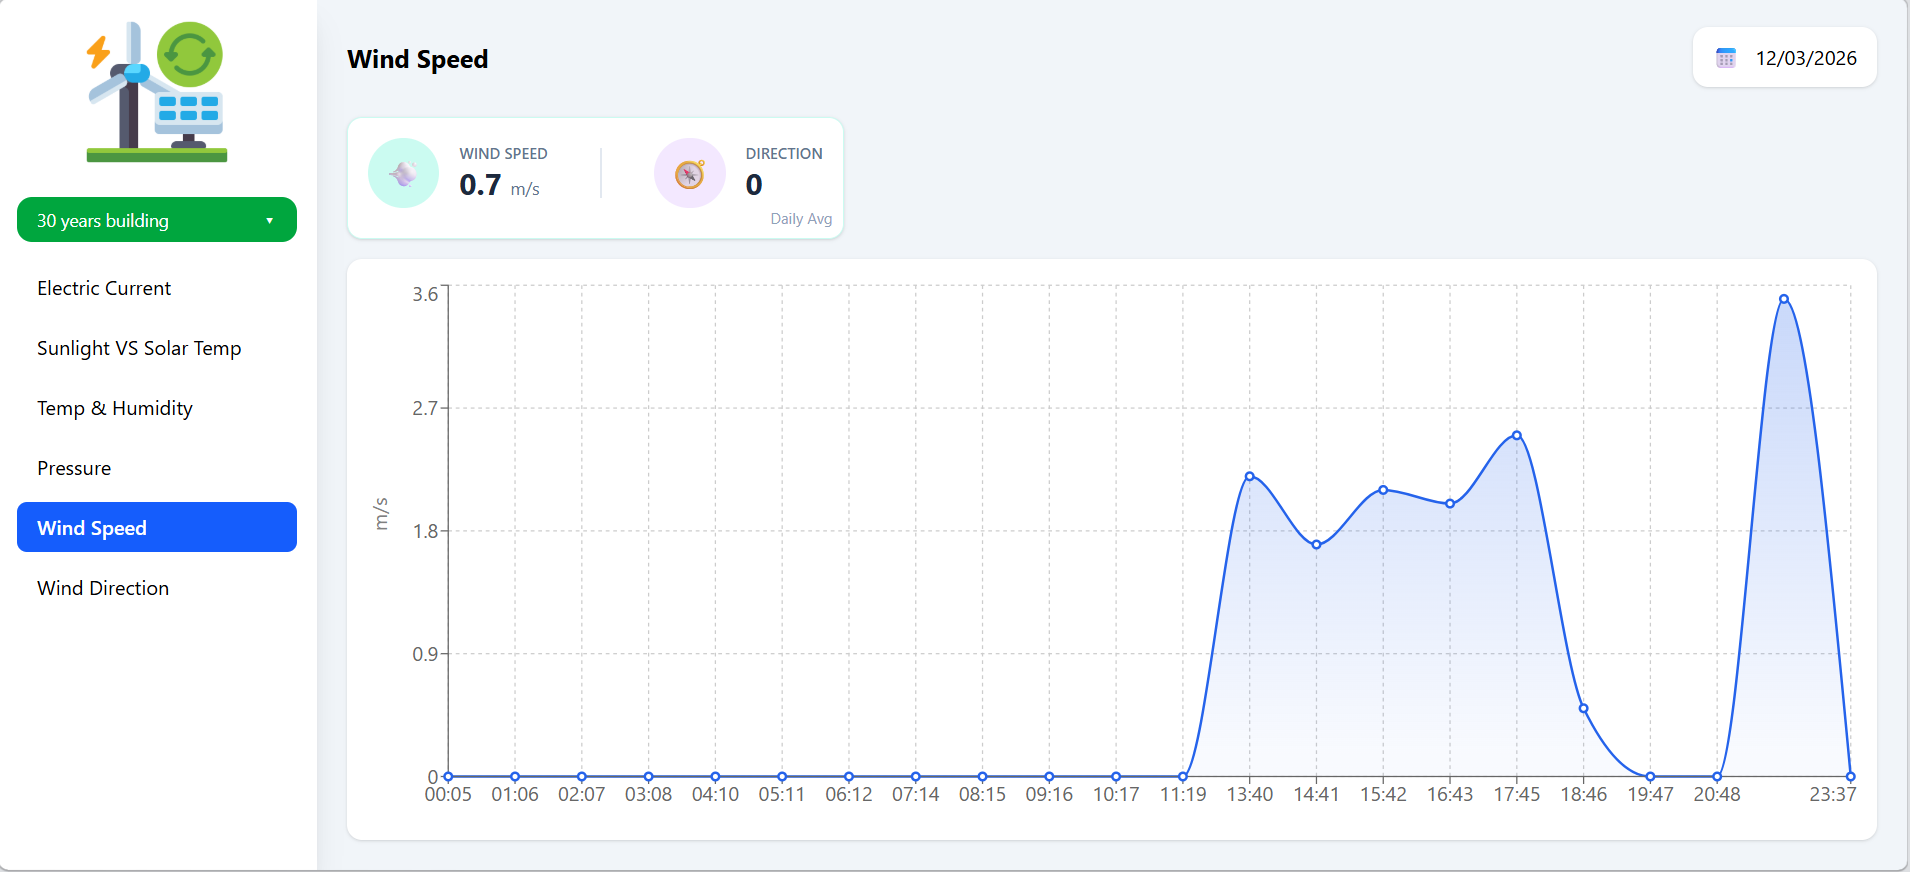
\includegraphics[width=0.7\textwidth]{picture/Wind Speed.png}
\caption[หน้าแสดงข้อมูลความเร็วลม]{หน้าแสดงข้อมูลความเร็วลม}
\label{fig:image10}
\end{figure}

\vspace{10pt}
\begin{itemize}
    \item แสดงข้อมูลความเร็วลมเฉลี่ยรายวัน 
    \item แสดงกราฟความเร็วลมในแต่ละช่วงเวลาของวัน เพื่อใช้เป็นข้อมูลประกอบในการวิเคราะห์ปัจจัยการระบายความร้อนของแผงโซลาร์เซลล์
\end{itemize}

\subsection{หน้าแสดงข้อมูลทิศทางลม}

\begin{figure}[H]
\centering
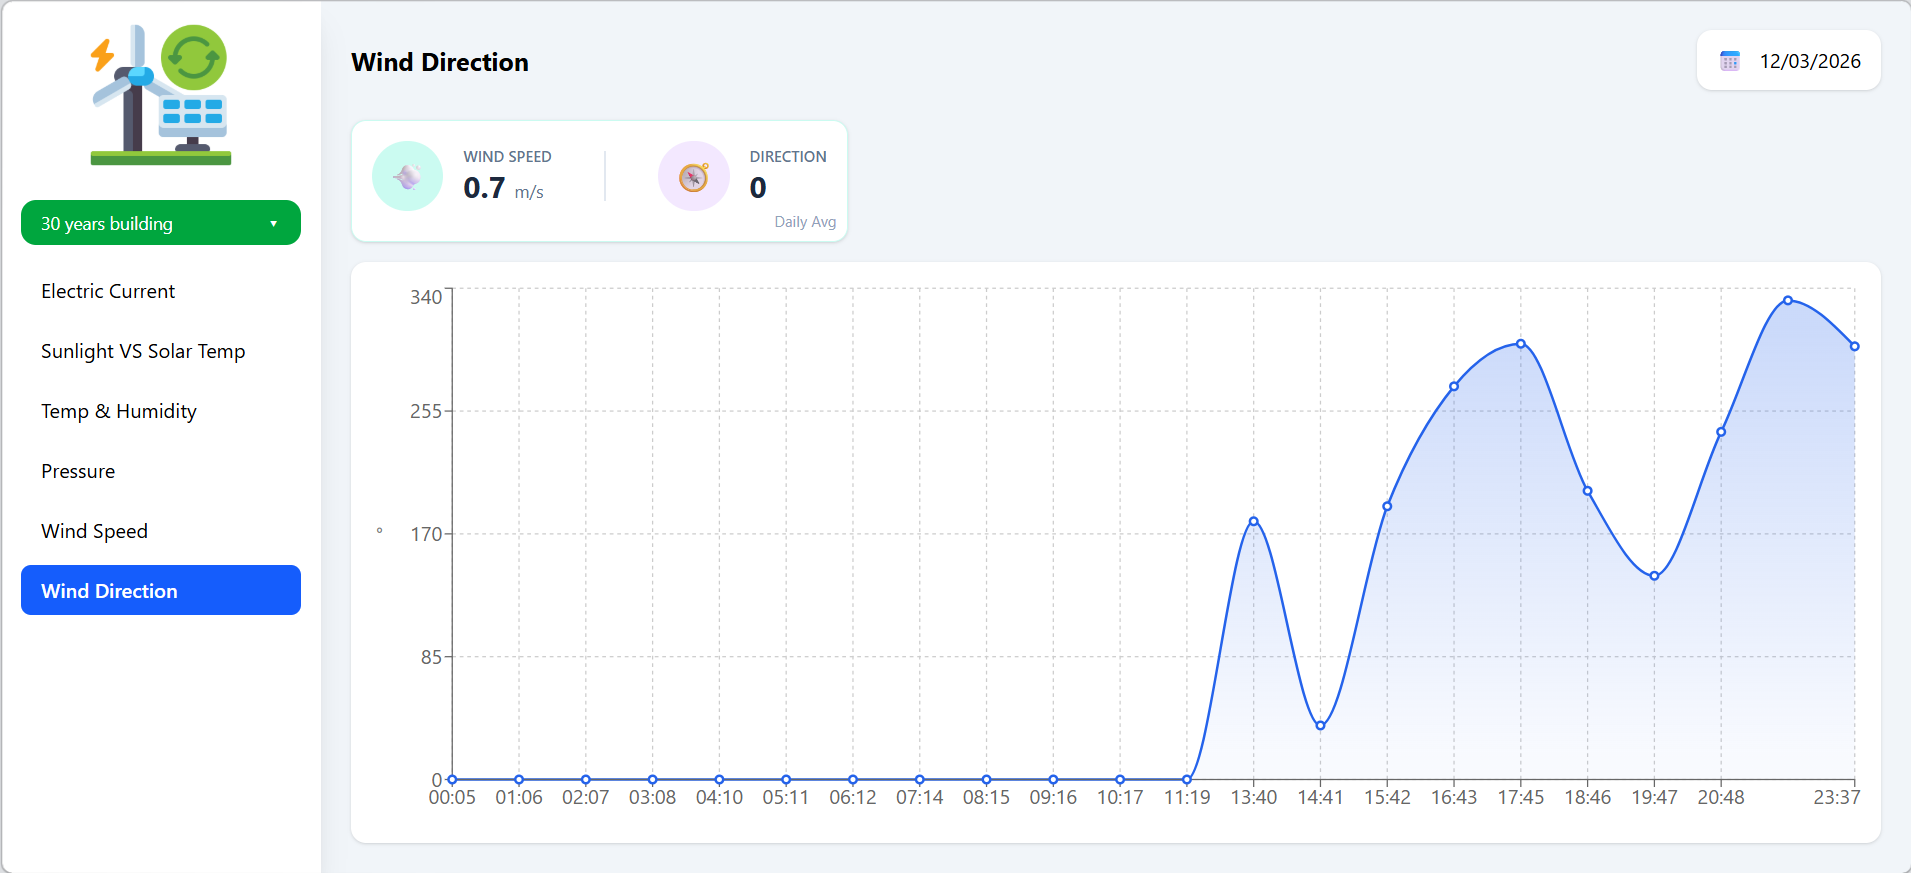
\includegraphics[width=0.7\textwidth]{picture/Wind Direction.png}
\caption[หน้าแสดงข้อมูลทิศทางลม]{หน้าแสดงข้อมูลทิศทางลม}
\label{fig:imag11}
\end{figure}

\begin{itemize}
    \item แสดงข้อมูลทิศทางลมเฉลี่ยรายวัน 
    \item แสดงกราฟการเปลี่ยนแปลงทิศทางลมในหน่วยองศาในแต่ละช่วงเวลาของวัน
\end{itemize}

\subsection{หน้าแสดงสถานะการทำงานของเซ็นเซอร์}

\begin{figure}[H]
\centering
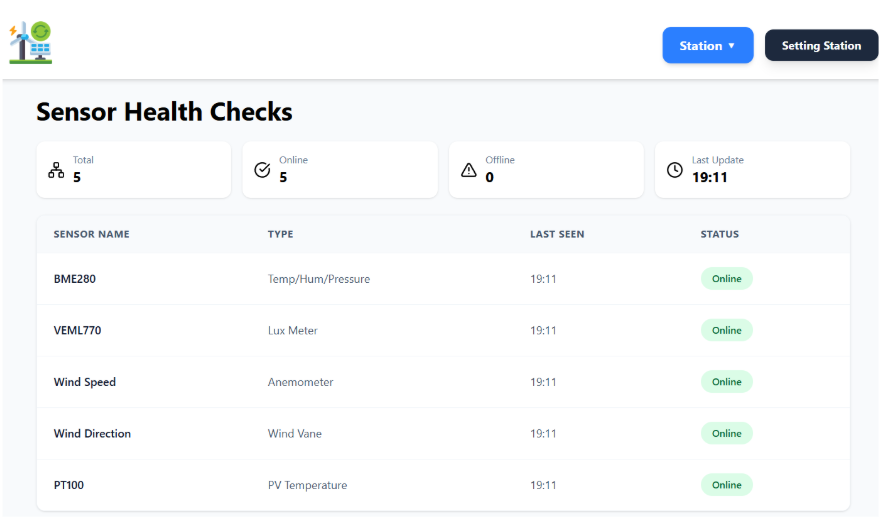
\includegraphics[width=0.7\textwidth]{picture/sensor check.png}
\caption[หน้าแสดงสถานะการทำงานของเซ็นเซอร์]{หน้าแสดงสถานะการทำงานของเซ็นเซอร์}
\label{fig:image12}
\end{figure}

\vspace{10pt}
\begin{itemize}
    \item แสดงข้อมูลภาพรวมต่างๆ ได้แก่ จำนวนเซ็นเซอร์ทั้งหมด จำนวนเซ็นเซอร์ที่ทำงานได้ปกติ จำนวนเซ็นเซอร์ที่ขาดการเชื่อมต่อ และเวลาที่ระบบได้รับการอัปเดตข้อมูลล่าสุด 
    \item แสดงรายละเอียดของอุปกรณ์แต่ละตัว ได้แก่ ชื่อเซ็นเซอร์ ประเภทการตรวจวัด เวลาที่ส่งข้อมูลเข้าเซิร์ฟเวอร์ครั้งล่าสุด และ สถานะการทำงาน 
    \item แสดงกราฟปริมาณการผลิตไฟฟ้าที่เกิดขึ้นจริงแบบรายชั่วโมง
    \item ผู้ใช้สามารถตรวจสอบสถานะการทำงานของเซ็นเซอร์ภายในสถานีวัดสภาพอากาศขนาดย่อมได้อย่างรวดเร็ว ซึ่งช่วยให้ง่ายต่อการซ่อมบำรุงเมื่ออุปกรณ์ตัวใดตัวหนึ่งเกิดปัญหา
\end{itemize}

\section{การประเมินความพึงพอใจในการใช้งานระบบ}

\hspace*{0.5cm}
ได้ทําการประเมินความพึงพอใจในการใช้งานระบบ โดยมีนักศึกษามหาวิทยาลัยเชียงใหม่ 21 คนทําการประเมินโดยแบ่งเป็นผู้ชาย 10 คน และผู้หญิง 11 คน โดยให้คะแนนในแต่ละหัวข้อการประเมินตามความพึงพอใจในการใช้งานระบบ ซึ่งผลการประเมินมีดังนี้
\begin{table}[H]
\centering
\renewcommand{\arraystretch}{1.5}
\begin{tabular}{|l|c|}
\hline
\textbf{หัวข้อการประเมิน} & \textbf{ความพึงพอใจ(เต็ม 5 คะแนน)} \\ \hline
ด้านการออกแบบเว็บไซต์ (Interface Design) & 4.84 \\ \hline
ด้านการแสดงผลข้อมูล (Data Visualization)   & 4.72 \\ \hline
ด้านการใช้งานระบบ (Usability)   & 4.71 \\ \hline
ด้านประสิทธิภาพของระบบ (System Performance)   & 4.67  \\ \hline
ด้านประโยชน์ของระบบ (Usefulness) & 4.84  \\ \hline
การเข้าถึงระบบ (Accessibility) & 4.80  \\ \hline
\end{tabular}
\caption{ตารางสรุปการประเมินความพึงพอใจในการใช้งานระบบ}
\label{tab:satisfaction}
\end{table}
\vspace{10pt}
\begin{flushleft}
\hspace*{0.5cm}
จากผลการประเมินความพึงพอใจรวมของผู้ทดลองใช้เว็บไซต์คือ 4.77 คะแนนหรือคิดเป็น 95.34\%
\end{flushleft}

Web Dashboard ที่พัฒนาขึ้นสามารถแสดงข้อมูลได้ถูกต้อง ผู้ใช้สามารถตรวจสอบข้อมูลสภาพอากาศ กราฟความสัมพันธ์ และผลการพยากรณ์ไฟฟ้าล่วงหน้าได้อย่างสะดวก โดยผลการประเมินความพึงพอใจเฉลี่ยอยู่ที่ 4.77 คะแนน หรือคิดเป็น 95.34\% สะท้อนให้เห็นว่าระบบช่วยให้ผู้ใช้งานเข้าถึงข้อมูลได้ง่าย และมีประโยชน์ต่อการวางแผนการใช้งานพลังงาน

โมเดลพยากรณ์ ผลการประเมินเชิงตัวเลขให้ค่า $R^2$ = 0.8619 และ MAE = 2.427 kWh แสดงว่าโมเดลมีประสิทธิภาพที่ดีสำหรับข้อมูลทดสอบที่เตรียมไว้ อย่างไรก็ตาม เมื่อนำไปใช้งานกับข้อมูลจริงพบว่าความคลาดเคลื่อนเฉลี่ยประมาณ 4.574 kWh เนื่องจากข้อมูลฝึกไม่ได้ใช้ข้อมูลที่ได้มาจากสถานีวัดสภาพอากาศที่ตั้งขึ้น รวมถึงปัจจัยแสงแดดและสภาพอากาศที่แปรผันแบบฉับพลันที่โมเดลอาจจะยังไม่สามารถเรียนรู้ได้ นอกจากนี้กราฟ Actual vs Predicted และ Residual Plot ยังแสดงให้เห็นว่าโมเดลมีความแม่นยำมากในช่วงกำลังผลิตระดับปานกลาง แต่มีความคลาดเคลื่อนเพิ่มขึ้นในช่วงกำลังผลิตสูง ซึ่งเป็นช่วงที่สภาพแสงไม่คงที่มากที่สุด

โดยสรุป ระบบทั้งหมดสามารถทำงานร่วมกันได้อย่างสมบูรณ์ ตั้งแต่การเก็บข้อมูล การประมวลผล การพยากรณ์ และการนำเสนอผลลัพธ์ แม้ว่าจะมีข้อจำกัดด้านปริมาณข้อมูลจริงและสภาพแวดล้อมที่มีความแปรผันสูง แต่ระบบถือว่ามีประสิทธิภาพที่ดีและมีความพึงพอใจจากผู้ใช้งานสูง ซึ่งสามารถนำไปประยุกต์ใช้ในการวางแผนการบริหารจัดการพลังงานภายในอาคารได้อย่างมีประสิทธิภาพ

